\documentclass[]{article}
\usepackage{lmodern}
\usepackage{amssymb,amsmath}
\usepackage{ifxetex,ifluatex}
\usepackage{fixltx2e} % provides \textsubscript
\ifnum 0\ifxetex 1\fi\ifluatex 1\fi=0 % if pdftex
  \usepackage[T1]{fontenc}
  \usepackage[utf8]{inputenc}
\else % if luatex or xelatex
  \ifxetex
    \usepackage{mathspec}
  \else
    \usepackage{fontspec}
  \fi
  \defaultfontfeatures{Ligatures=TeX,Scale=MatchLowercase}
\fi
% use upquote if available, for straight quotes in verbatim environments
\IfFileExists{upquote.sty}{\usepackage{upquote}}{}
% use microtype if available
\IfFileExists{microtype.sty}{%
\usepackage{microtype}
\UseMicrotypeSet[protrusion]{basicmath} % disable protrusion for tt fonts
}{}
\usepackage[margin=1in]{geometry}
\usepackage{hyperref}
\hypersetup{unicode=true,
            pdfborder={0 0 0},
            breaklinks=true}
\urlstyle{same}  % don't use monospace font for urls
\usepackage{graphicx,grffile}
\makeatletter
\def\maxwidth{\ifdim\Gin@nat@width>\linewidth\linewidth\else\Gin@nat@width\fi}
\def\maxheight{\ifdim\Gin@nat@height>\textheight\textheight\else\Gin@nat@height\fi}
\makeatother
% Scale images if necessary, so that they will not overflow the page
% margins by default, and it is still possible to overwrite the defaults
% using explicit options in \includegraphics[width, height, ...]{}
\setkeys{Gin}{width=\maxwidth,height=\maxheight,keepaspectratio}
\IfFileExists{parskip.sty}{%
\usepackage{parskip}
}{% else
\setlength{\parindent}{0pt}
\setlength{\parskip}{6pt plus 2pt minus 1pt}
}
\setlength{\emergencystretch}{3em}  % prevent overfull lines
\providecommand{\tightlist}{%
  \setlength{\itemsep}{0pt}\setlength{\parskip}{0pt}}
\setcounter{secnumdepth}{0}
% Redefines (sub)paragraphs to behave more like sections
\ifx\paragraph\undefined\else
\let\oldparagraph\paragraph
\renewcommand{\paragraph}[1]{\oldparagraph{#1}\mbox{}}
\fi
\ifx\subparagraph\undefined\else
\let\oldsubparagraph\subparagraph
\renewcommand{\subparagraph}[1]{\oldsubparagraph{#1}\mbox{}}
\fi

%%% Use protect on footnotes to avoid problems with footnotes in titles
\let\rmarkdownfootnote\footnote%
\def\footnote{\protect\rmarkdownfootnote}

%%% Change title format to be more compact
\usepackage{titling}

% Create subtitle command for use in maketitle
\newcommand{\subtitle}[1]{
  \posttitle{
    \begin{center}\large#1\end{center}
    }
}

\setlength{\droptitle}{-2em}
  \title{}
  \pretitle{\vspace{\droptitle}}
  \posttitle{}
  \author{}
  \preauthor{}\postauthor{}
  \date{}
  \predate{}\postdate{}


\begin{document}

\chapter[Renfrewshire Council Exploratory Project]{Renfrewshire Council \\ Exploratory Project}\label{ch:renfrew}

\section{Introduction}\label{renf-intro}

As described in Chapter \ref{ch:data}, the Social Care Survey (SCS) is
collected annually by the Scottish Government and provides a snapshot of
individuals receiving social care in all 32 Scottish local authorities
during a census week - usually including the date the 31st of March
(Scottish-Government 2017c). The cross-sectional nature of this
adminsitrative data means it does not identify every individual who
receives social care in any given financial year. This has implications
for the interpretation of research projects using the SCS and the
statistical inferences that can be applied to the data when linked with
other sources of information.

In order to gain a better understanding of the data the SCS captures
(and the data it does not) an exploratory study was conducted to assess
social care data for individuals from one local authority only. This
project aimed to analyse complete data for all individuals over a
ten-year period to assess the validity of the SCS as a representation of
social care delivered in any given financial year. In particular, the
exploratory analysis aimed to; quantify the proportion of home care
users identified by the SCS in each year, identify what differences (if
any) exist between home care packages captured and not captured by the
census, and assess whether values captured by the SCS (i.e.~the total
hours of home care provided) are representative of care received by an
individual throughout the year. Given intentions to amalgamate the SCS
with administrative resources collected by ISD and move to a quarterly
collection of data (ISD 2017), the exploratory project also aimed to
quantify the proportion of all individuals that would be identified by
two, three, or four survey repetitions per financial year.

As social care data in Scotland has rarely been used for research
purposes, this exploratory project also offered the opportunity to
assess the format, content, and suitability of the data from a research
perspective. Ideally, data would be analysed from a number of local
authorities for comparison. However, as described below, acquiring
sensitive data of this nature is a lengthy and complicated process,
relying heavily on the goodwill of the participating local authority.
Despite early intentions to approach multiple local authorities,
practical considerations limited the project to data collected from
Renfrewshire Council.

SCS umbrella and breakdown with Renfrew data

\section{Background}\label{sec:renf-background}

The decision to approach Renfrewshire Council as a potential source of
data was due to convenience given previous cooperation between the
council and UBDC on other projects. Another local authority was also
approached but preliminary discussions suggested that whilst the purpose
of proposed research was supported, the council was unlikely to be able
to provide sufficient resource to facilitate data sharing. Preliminary
meetings with data analysts from Renfrewshire council confirmed that
data could be provided to facilitate the proposed research and the
formal process of obtaining data using UBDC's controlled data service
was instigated in April 2016.

Renfrewshire Council area accounts for 3.2\% of the total population of
Scotland and has a similar proportion of individuals aged over 60
compared to the rest of the country (24.4\% v 24.2\%) (NRS 2015). The
mortality rate is very slightly higher than recorded for the rest of
Scotland (10.9\% v 10.3\%) with the main causes of death being cancer,
circulatory diseases, and respiratory diseases (NRS 2015). Life
expectancy at birth is lower than the Scottish average for both males
and females (75.9 v 77.1 \& 80.6 v 81.1) (NRS 2015). Sixty-three percent
of dwellings in Renfrewshire fall into the lowest council tax bands A-C
(NRS 2015) which is a higher than the ratio seen in the whole country
(61\%) (NRS 2016). Of all datazones in the Renfrewshire Council area,
37.3\% fall into the most deprived 30\% of Scottish datazones - the
ninth highest rate out of all 32 local authorities (Scottish-Government
2017a). Datazones in the area show marked differences in SIMD scores
with some of the most and least deprived datazones in the whole of
Scotland and a spread of urban and rural neighbourhoods
(Scottish-Government 2017a).

In terms of social care, the 2017 SCS (Scottish-Government 2017b,
supp.charts) shows that the proportion of over 65s receiving home care
provided or administered by Renfrewshire dipped a little between 2011
and 2015 but has nearly returned to 2010 levels (52.4 per thousand in
2010, 49.4 per thousand in 2017). Historically, this is lower than
levels seen across Scotland as a whole, although national levels are now
very similar to those seen in Renfrew (60.8 per thousand in 2010 to 48.9
per thousand in 2017). The absolute numbers of over 65s receiving home
care in Renfrewshire in the 2010 census week was 1812 versus 1603 in the
2017 census (Scottish-Government 2017b, supp.charts).

More recent versions of the SCS collect information on home care (such
as personal care or reablement), housing support and meals services
provided during the census week. In addition, data on services such as
community alarm, telecare, social worker, and self-directed support that
are provided at any time during the financial year is also collected
(Scottish-Government 2017b). The purpose of the exploratory project was
to compare service provision of those services collected in the census
week. As the vast majority of this data is focussed on home care
services, the analysis concentrates on this service only. Home care
refers to services received in the home such as personal care or
reablement (described in section \ref{subsec:access-sc-defs} ans
summarised in table \ref{tab:renf-homecaredefs}).

\begin{table}[]
\centering
\caption{Definitions of home care types}
\label{tab:renf-homecaredefs}
\resizebox{\textwidth}{!}{%
\begin{tabular}{@{}ll@{}}
\toprule
\textbf{Type of home care} & \textbf{Definition} \\ \midrule
Care at Home (Mainstream & \begin{tabular}[c]{@{}l@{}}The aim of care at home is to help vulnerable people of all ages live independently and securely in their\\  own homes by providing personal and housing support services. Care at home services are provided very\\  much on each individual's own circumstances and needs.\end{tabular} \\ \midrule
Reablement & \begin{tabular}[c]{@{}l@{}}Provides support and encouragement to help keep up or increase the skills and confidence needed \\ to be able to return home after a stay in hospital or after an illness.Most people referred for care at \\ home will receive a reablement service in the first instance to help support and improve independence.\\ Long term services can be provided following reablement if ongoing support is needed.\end{tabular} \\ \midrule
Rapid Response &  \\ \midrule
Community Mental Health & \\ \midrule
Extra Care Housing &  \\ \midrule
Housing Support & \\ \midrule
Overnight Services & \\ \bottomrule
\end{tabular}%
}
\end{table}

\FloatBarrier
\subsection{Research Questions}\label{subsec:renfrew-qs}

\begin{itemize}[noitemsep]
\item To what extent does SCS data capture the distribution of individuals receiving home care across each financial year?
\item Are there differences in the types of home care package that are/are not captured by the census? Do these differences vary by age or gender?
\item For packages that \emph{are} captured by the SCS, is the value of total hours of home care received reflective of the total hours of home care received in the previous and following six months?
\item What proportion of the total amount indiviudals receiving home care would be captured if more than one census was conducted in each financial year?
\end{itemize}

\section{Methods}\label{sec:renf-methods}

\subsection{Project approvals and timeline}\label{subsec:renf-methods-approvals}

The exploratory project utilised the controlled data service provided by
UBDC and therefore required approval from UBDC's Research Approvals
Committee (RAC). This process is more fully explained in section
\ref{subsec:rac} Approval from RAC was gained on 01/06/2016
\emph{(Appendix A)}. Ethical approval for the study was gained from the
University of Glasgow College of Social Sciences Research Ethics
Committee on 24/05/2016 \emph{(Appendix B)}. .

Following academic and ethical approval the process of obtaining a data
sharing agreement (DSA) between the University of Glasgow and
Renfrewshire council was instigated. This involved the production of an
agreement in principal and privacy impact assessment as a basis for the
DSA. Production of the DSA involved the input of legal teams from both
institutions as well as liaison with data analysts at Renfrewshire
council and UBDC. The initial draft was produced by the local authority
with amendments from both sides before final completion and signing
06/09/2017. Final transfer of data took place on 21/09/2017. An
illustration of this timeline is shown in figure \ref{fig:ren-timeline}

\begin{figure}[h]
  \centering
    \caption{Timeline of Renfrewshire exploratory project}
    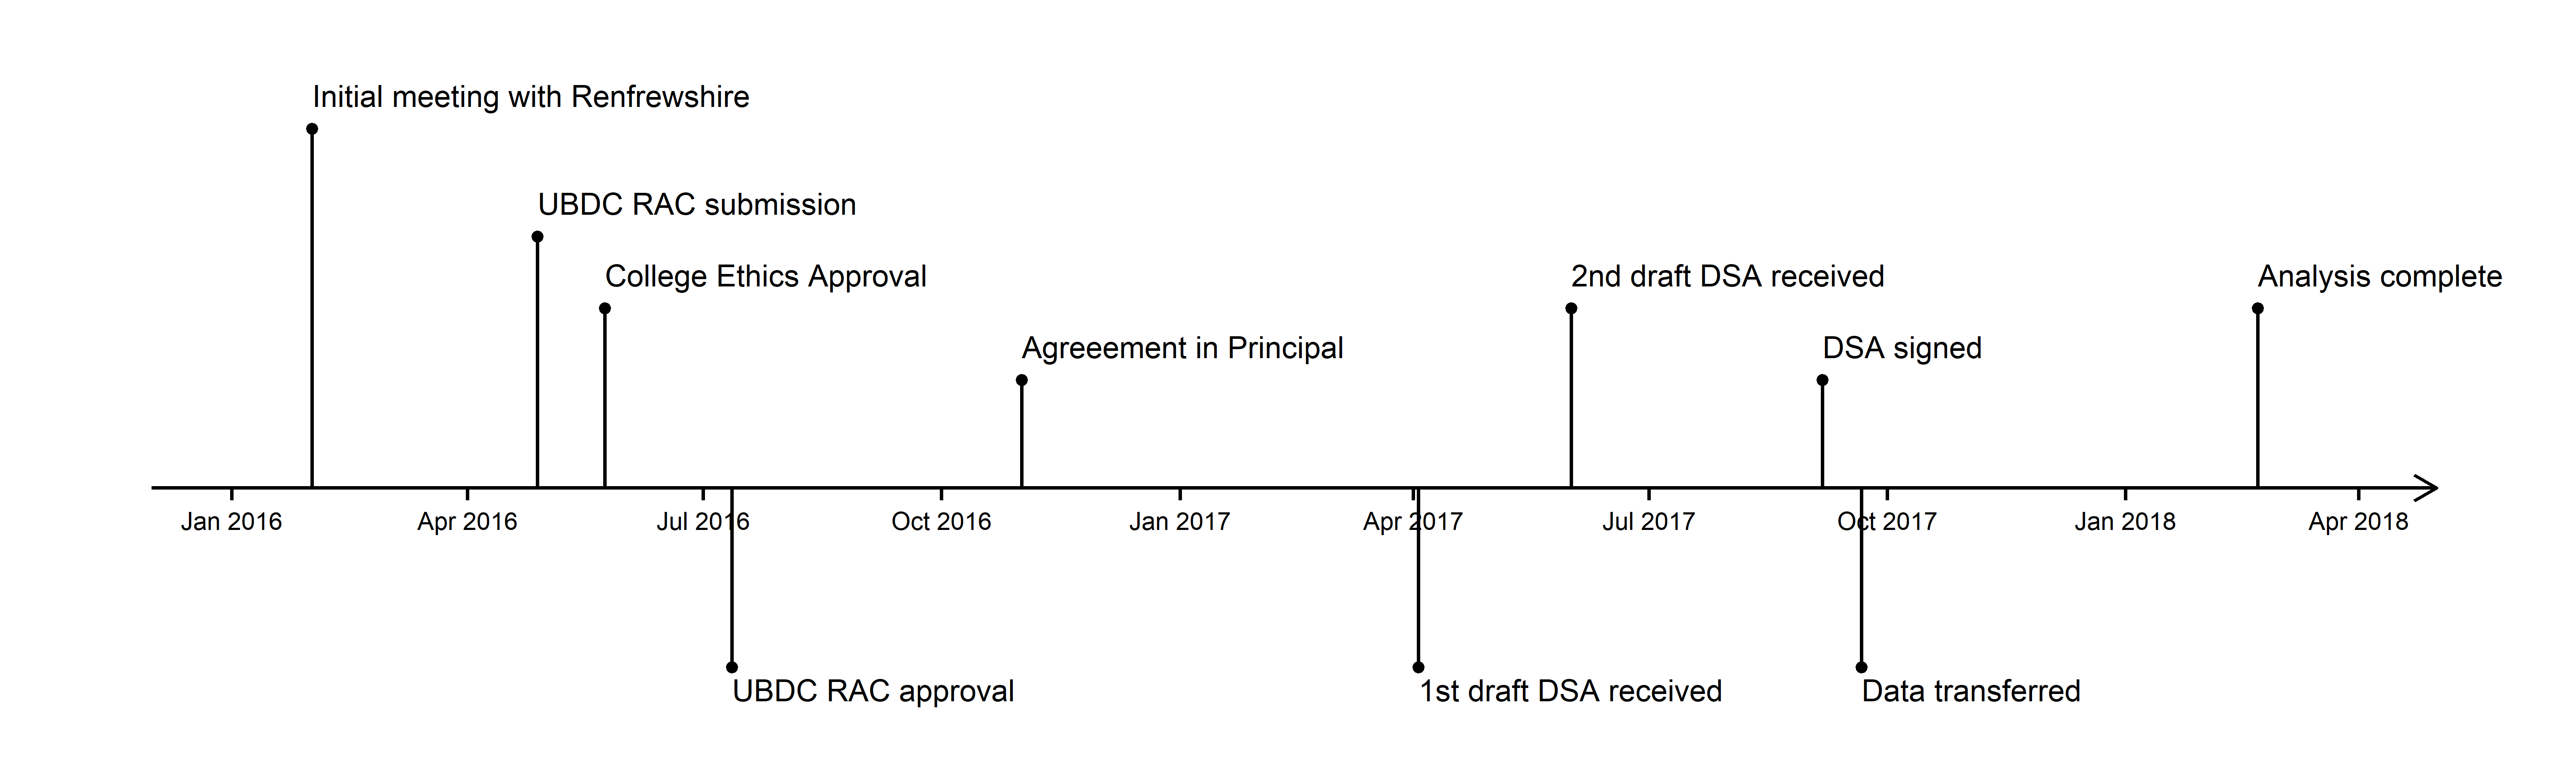
\includegraphics{figures/chapter-renf/renf-timeline.png}
    \label{fig:ren-timeline}
\end{figure}

\subsection{Data}\label{subsec:renf-methods-data}

As with all services provided by Renfrewshire council, home care data is
collected to ensure efficient management of the service and as evidence
of service provision (Renfrewshire-Council 2015). Recording of
individual episodes of care also helps with budgetary management of the
service.

Data provided for the purposes of this exploratory study detailed
anonymised information on; how many days per week, how many hours per
day, service provider (e.g.~local authority or independent provider),
type of care (e.g.~mainstream or reablement), start date and end date
for every episode of home care delivered to individuals in the
Renfrewshire council area between April 2006 and April 2017. Demographic
information detailing gender and year of birth was also provided.

As all episodes of home care were delivered over a period of time, data
was provided for some packages where the care was first delivered as
early as 2004 or as late as Summer 2017 (e.g.~a home care episode
starting in December 2005 and running to December 2006 was included in
the data transfer). Data detailing information on community alarm and
telecare services provided by Renfrewshire council were not analysed as
part of this project.

Analysis focussed on individuals over the age of 65. An unexpectedly
large number of individuals (n = 112, 0.01\%) had a year of birth
recorded as 1900 (compared to n = 68 born between the years 1901 and
1910). A similar phenomenon was reported in the SCS linkage process
(described in chapter \ref{ch:methods}) with the deduction that 1900 was
a code for missing data. In this analysis these records were omitted. To
protect anonymity individual month and day of birth were not shared
meaning age was calculable from year of birth only.

The SCS requests information on the total hours of home care each
individual received during the census week. To replicate this
information, every episode of care in the exploratory dataset was
summarised. For each episode of home care the number of hours per day
was multiplied with days per week to give a weekly total of home care
hours for each episode. To identify \emph{packages} of home care,
episodes of home care with the same start and end date and of the same
home care type, were added together. For example, an individual
receiving home care of the type ``Care at Home (Mainstream)'' with an
episode of care lasting 1 hour in the morning for 3 days a week, an
episode of care lasting 45 minutes at lunchtime 7 days a week, an
evening episode of 30 minutes 7 days a week, and nightime episode of 45
mins 7 days a week, would have a total weekly home care hours count of
17 hours per week for that home care type. Finally, the totals for all
types of home care were summed to give an overall weekly total for each
individual.

\subsection{Analysis}\label{subsec:renf-methods-analysis}

To enable comparison of packages at different time points a time-series
was created for the study period 27th March 2006 to 28th March 2016 at
weekly intervals. The value of total hours of home care each individual
was receiving at each of the 523 weekly time points was identified. From
this time series weekly counts of the total number of individuals
receiving home care were calculated. Maximum and minimum values,
measures of central tendency and range of these weekly values were
compared to the total number of individuals receiving home care in each
financial year and visualised. Comparison was also made of the number of
indivudals receving home care in the census week to figures returned by
Renfrewshire council to the SCS for the same census week.

For the financial years 2011/12 - 2015/16 (the study period of the main
thesis project) data was subset to identify those packages of home care
that were ``live'' during the week including the 31st of March and those
that were not ``live'' i.e. (those that would not have been captured by
SCS census). These subsets were then compared by visualising the
distribution of package duration and intensity (i.e.~the total hours of
homecare provided) across age and gender groups. The non-parametric
Mann\_Whitney U test was used to compare differences between groups with
p-values \textless{}0.05 accepted as showing a statistically significant
difference. As the home care packages of the types ``Community Mental
Health'', ``Overnight Services'', ``Housing Support'', and ``Extra Care
Housing'' accounted for less than one percent of packages of care, they
were omitted from the comparative visualisations and analysis.

In order to assess whether the value of the total hours of homecare
provided was representative of care in the six months preceding and
following the census week, data was subset by individuals who only
received a single package of care in the 12 months surrounding the
census and those that received multiple packages of care. For those that
received single packages of care, and therefore had an accurate
measurement of their total hours of care, the distribution of the
duration of these packages was assessed. For those that received mutiple
packages of care, and therefore had differing values of hours of home
care, the net difference in total hours of care received across all
packages was calculated in order to summarise the variation from the
reported hours of each individual. For example, an individual intially
receiving 6 hrs of care, experiencing a break in care to zero hours, and
then receiving a new package of care of 7 hrs before a further drop to 2
hrs would have a net difference of \((-6 + 7 - 5) = -4\) hours. The
distribution of this value across all individuals was then assessed.

Additional variables indicating whether home care packages were ``live''
at three, four, six, eight, and nine months before the census of each
financial year were appended to the dataset. This enabled counts of
indiviudals who would be captured by six-monthly, four monthly, and
three monthly census repetitions.

All data cleaning and analysis was conducted using the R language and
environment for statistical computing version 3.4.0 (R-Core-Team 2017)
with packages \texttt{dplyr} v0.7.4 (Wickham and Francois 2017),
\texttt{tidyr} v0.7.2. (Wickham and Henry 2017), \texttt{forcats} v0.2.0
(Wickham 2017), \texttt{purrr} v0.2.4 (Henry and Wickham 2017),
\texttt{lubridate} v1.6.0. (Grolemund and Wickham 2017),
\texttt{magrittr} v1.5 (Bache and Wickham 2014), \texttt{broom} v0.4.2
(Robinson 2017), and \texttt{ggplot2} v2.2.1 (Wickham and Chang 2016)
via the Integrated Development Environment RStudio v1.0.143
(RStudio-team 2016). Data was held securely in the safe haven
environment described in section \ref{subsec:safe-haven}

\FloatBarrier

\section{Results}\label{sec:renf-results}

\subsection{Descriptive statistics}\label{subsec:renf-descriptives}

After data cleaning, information on 41,002 packages of home care
received by 10,130 individuals during the period 2006 to 2016 were
included in the analysis. The number of records retained at each stage
of the cleaning process is shown in table \ref{tab:renf-cleaning}. Of
these packages, 28,775 described actual packages of care. The remainder
described placeholders for each individual where they were not receiving
care, either because of a break in care or beacuse care provision had
ended altogether. These 12,227 records showed a value of zero for the
total hours of homecare received and in the case of care provision
having ended, showed an end date of 28th March 2016.

\begin{table}[h]
\centering
\caption{Number of records at each stage of data cleaning}
\label{tab:renf-cleaning}
\begin{threeparttable}
\begin{tabular}{@{}lr@{}}
\toprule
Data Cleaning stage                & Number of records \\ \midrule
Initial home care file             & 106,111           \\
Including over 65s only            & 92,723             \\
Summarised to packages of care     & 41,002\tnote{1}    \\ 
Packages of non-zero hours of care & 28,775             \\ \bottomrule
\end{tabular}
\begin{tablenotes}
\item[1] Total number of indiviudals = 10,310
\end{tablenotes}
\end{threeparttable}
\end{table}

Mean age of those included in the analysis was 80.8 years and median age
was 81. Sixty-four percent of individuals (n = 6515) were female.
Detailed breakdown of age and gender groups is shown in figure
\ref{fig:ren-age-gen}. The highest absolute numbers of individuals are
found in the 76-85 age group. Statistical disclosure control meant that
grouping an additional age group for over 95s was not possible.

\begin{figure}[h]
  \centering
    \caption{Breakdown of age and gender}
    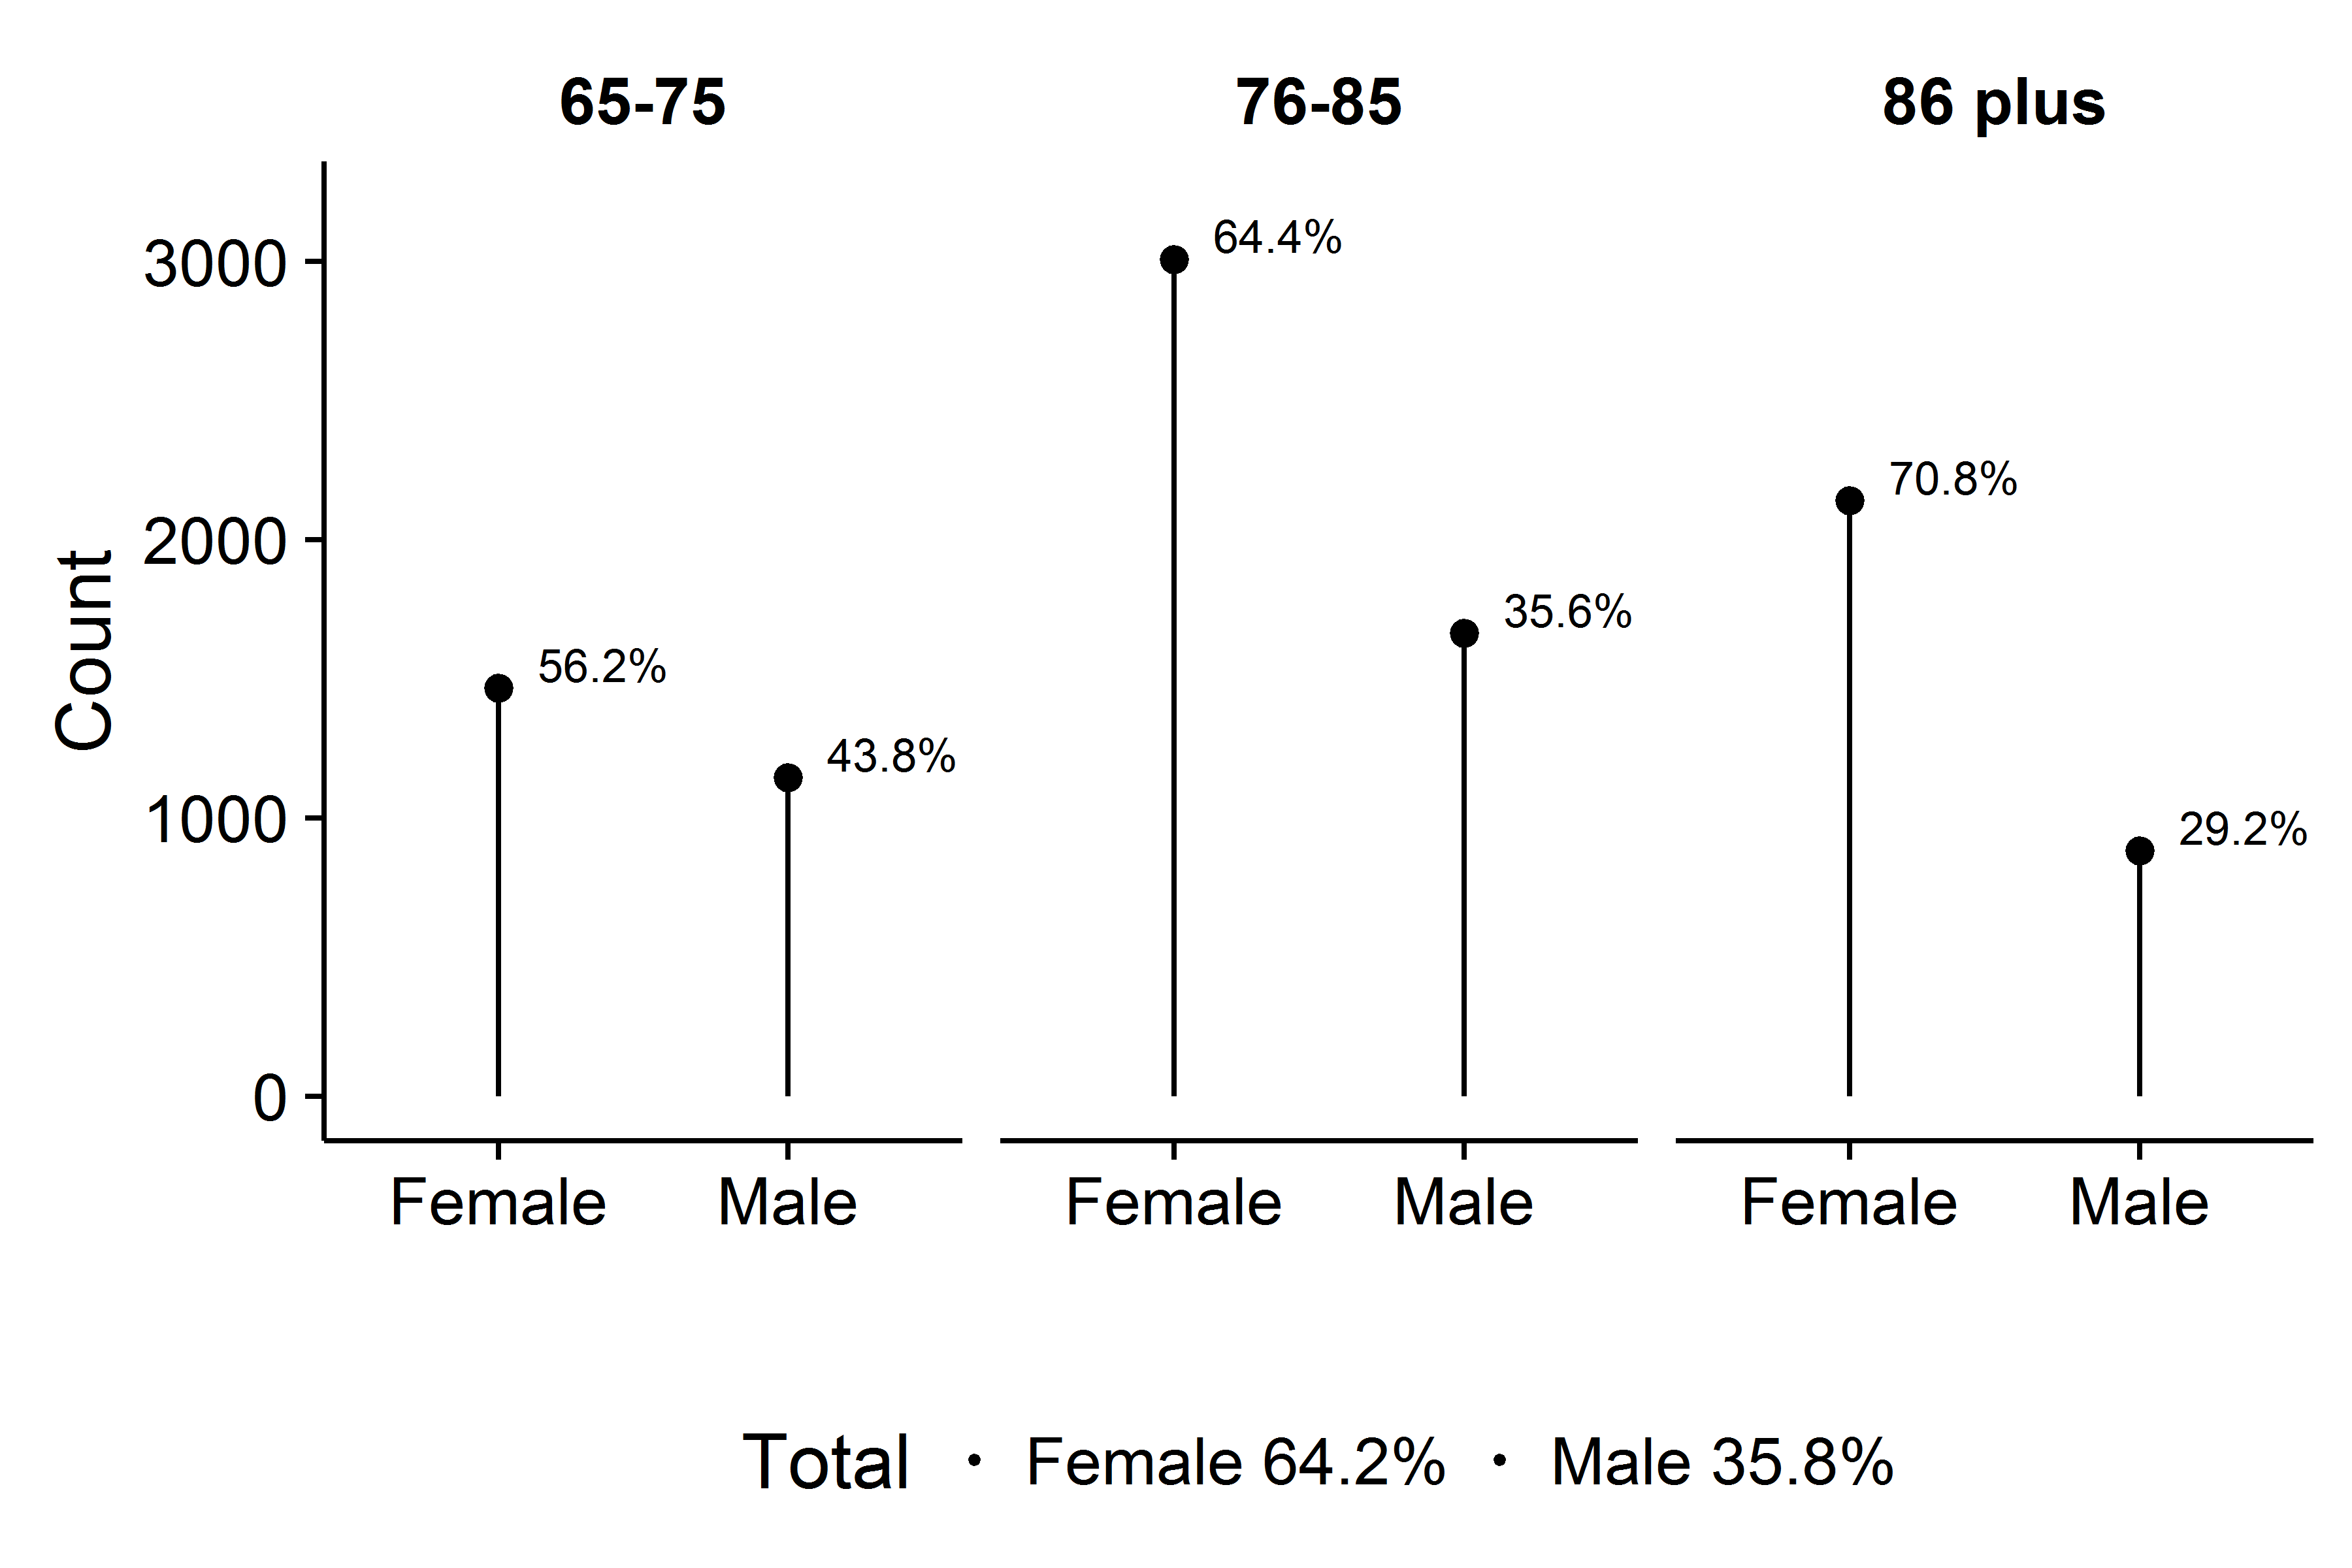
\includegraphics[height = 10cm, width = 12cm]{figures/chapter-renf/01-age-gender-ts-subset.png}
    \label{fig:ren-age-gen}
\end{figure}

Seventy-eight percent of home care packages (n=22484) were provided for
``Care at Home (Mainstream)'' with ``Reablement'' type packages making
up the majority of the remainder (Figure \ref{fig:ren-type}). Only 60
packages of care for over 65s were classified as being provided for
``Community Mental Health'' or ``Overnight Services'' during the study
period. ``Reablement'' packages were first coded as such in the
financial year 2010/11 meaning ``Care at Home (Mainstream)'' made up an
even larger proportion of care packages prior to this.

\begin{figure}[]
  \centering
    \caption{Count and proportion of home care type}
    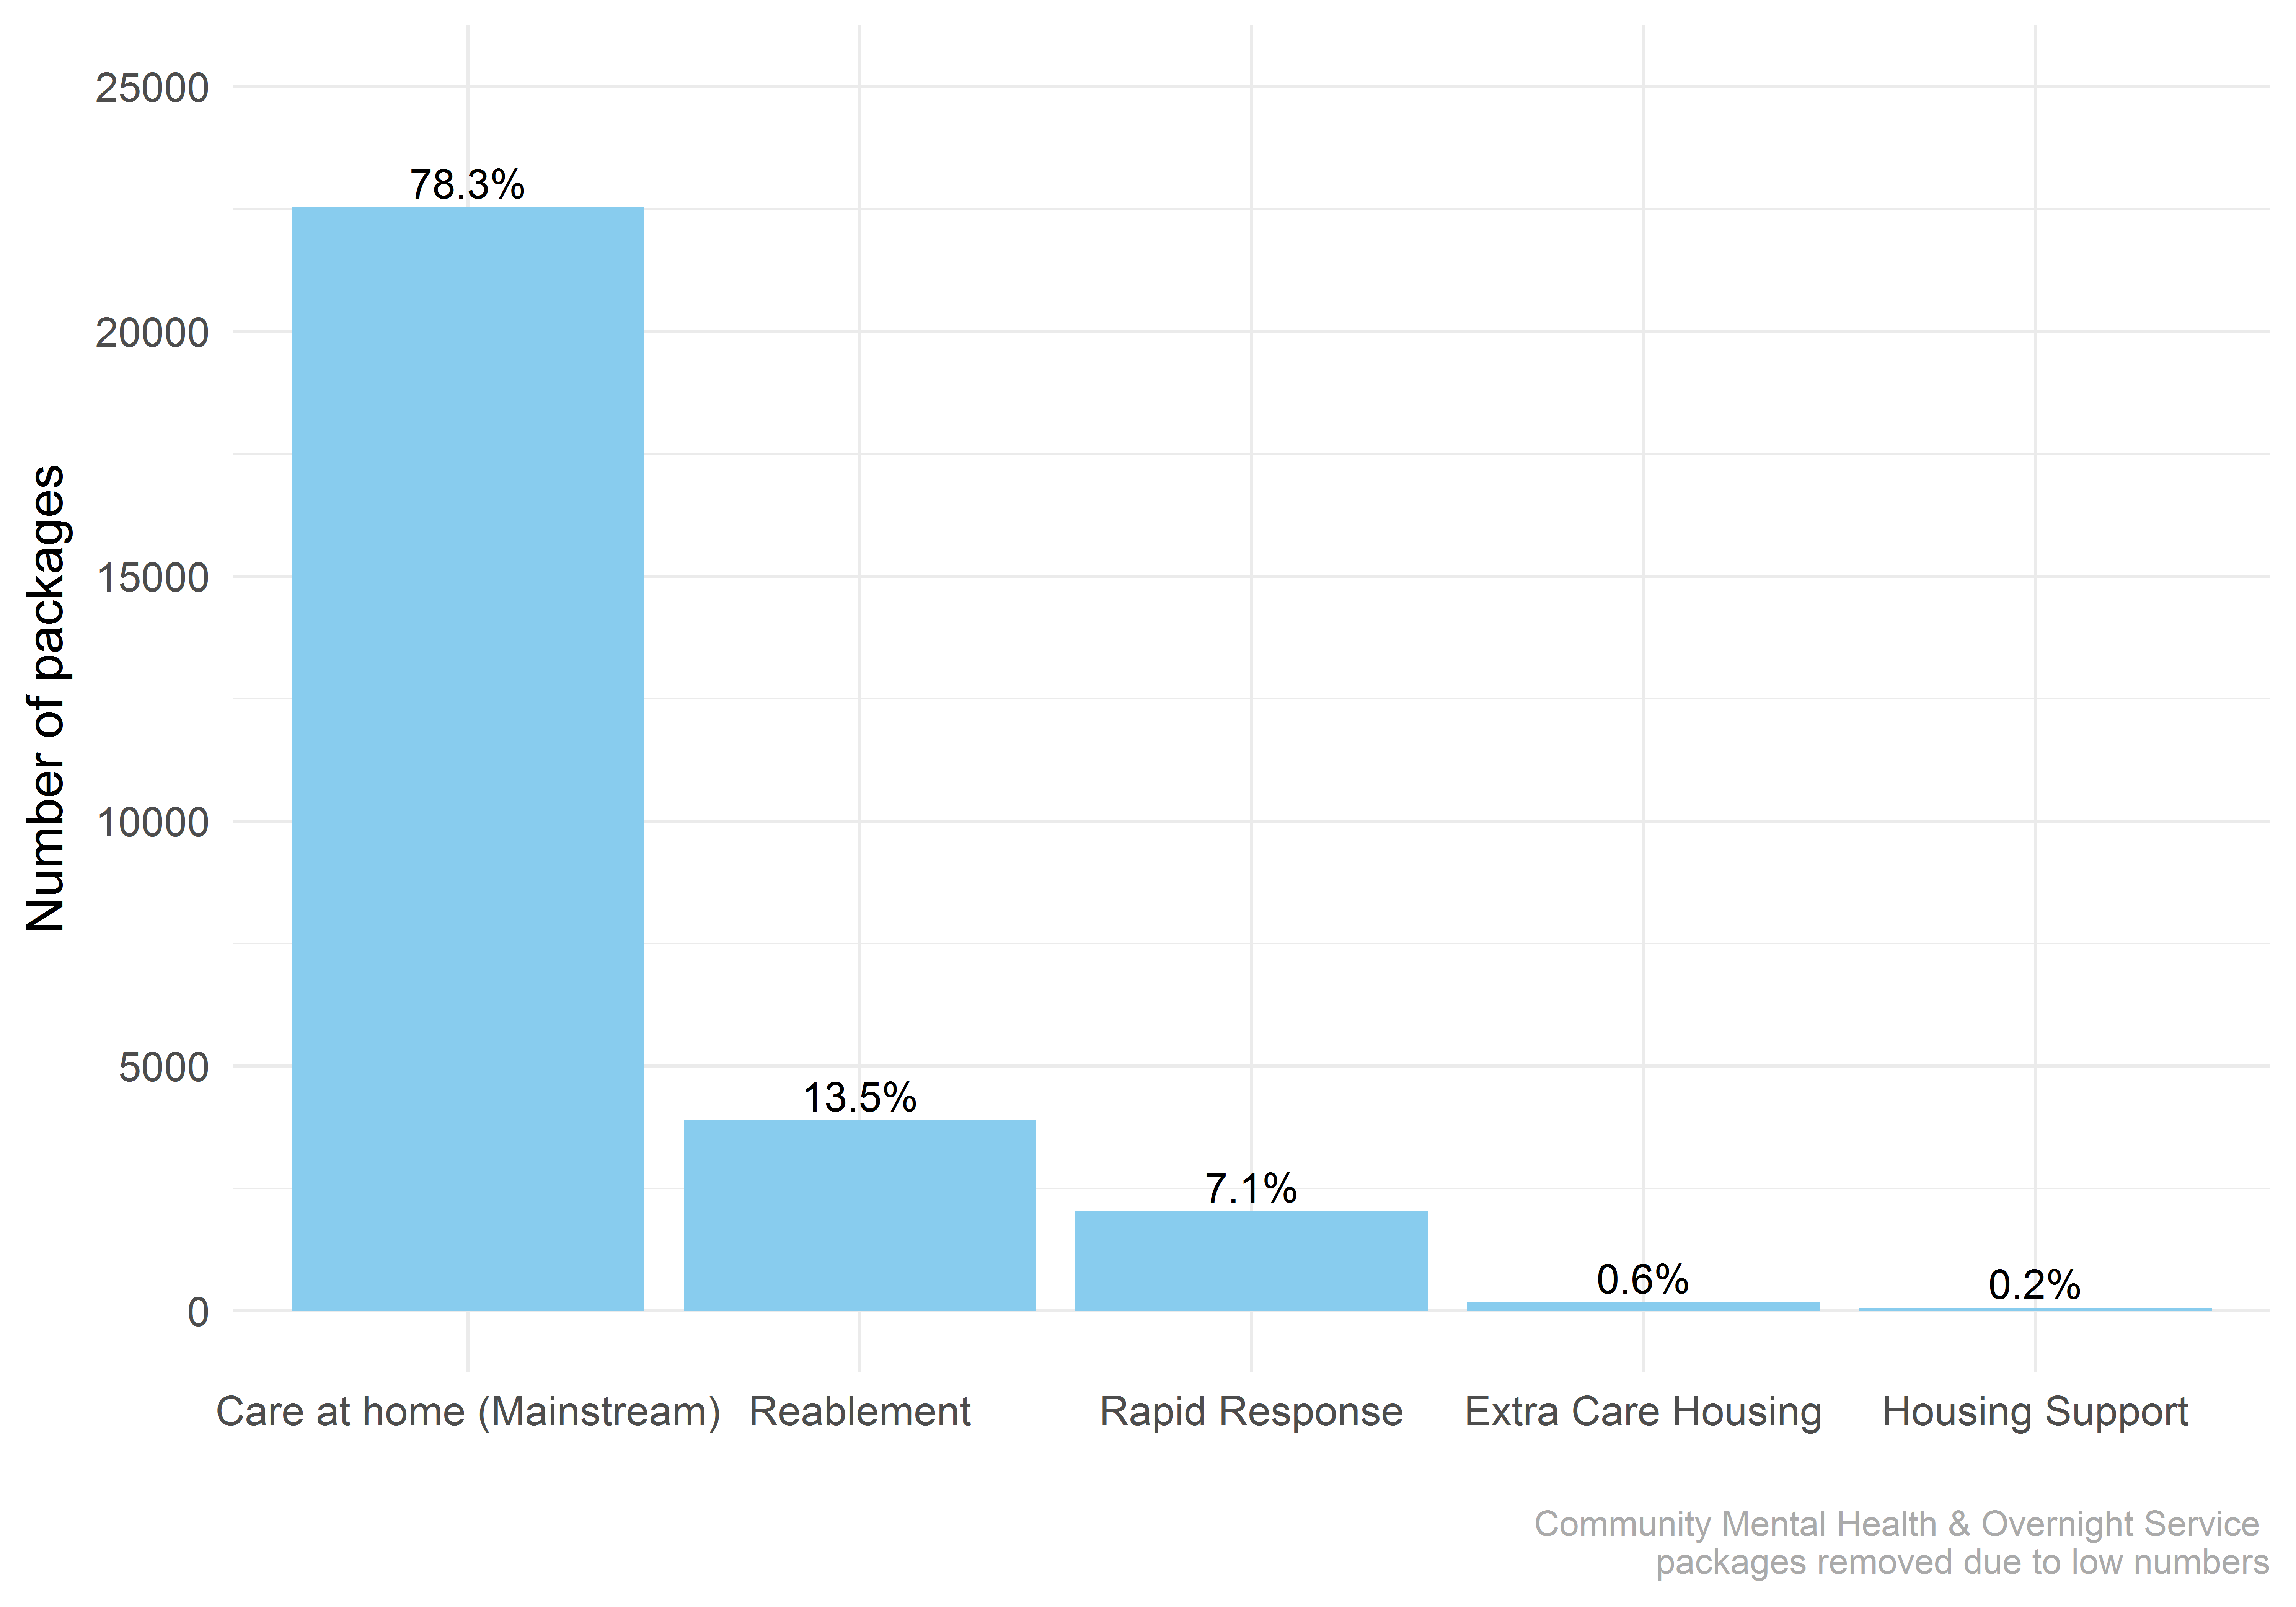
\includegraphics[height = 10cm, width = 12cm]{figures/chapter-renf/03-pack-plot}
    \label{fig:ren-type}
\end{figure}

Almost two-thirds of home care packages in the study period provided
care at intensities of less than 10 hours per week. Only 1,352 (47\%)
packages over the 10 year study period provided high intensity care of
over 20 hours per week (figure \ref{fig:ren-hrs}). Eight-five percent of
packages lasted for less than one year (figure \ref{fig:ren-duration}).

\begin{figure}[h]
  \centering
    \caption{Count of packages of care by intensity}
    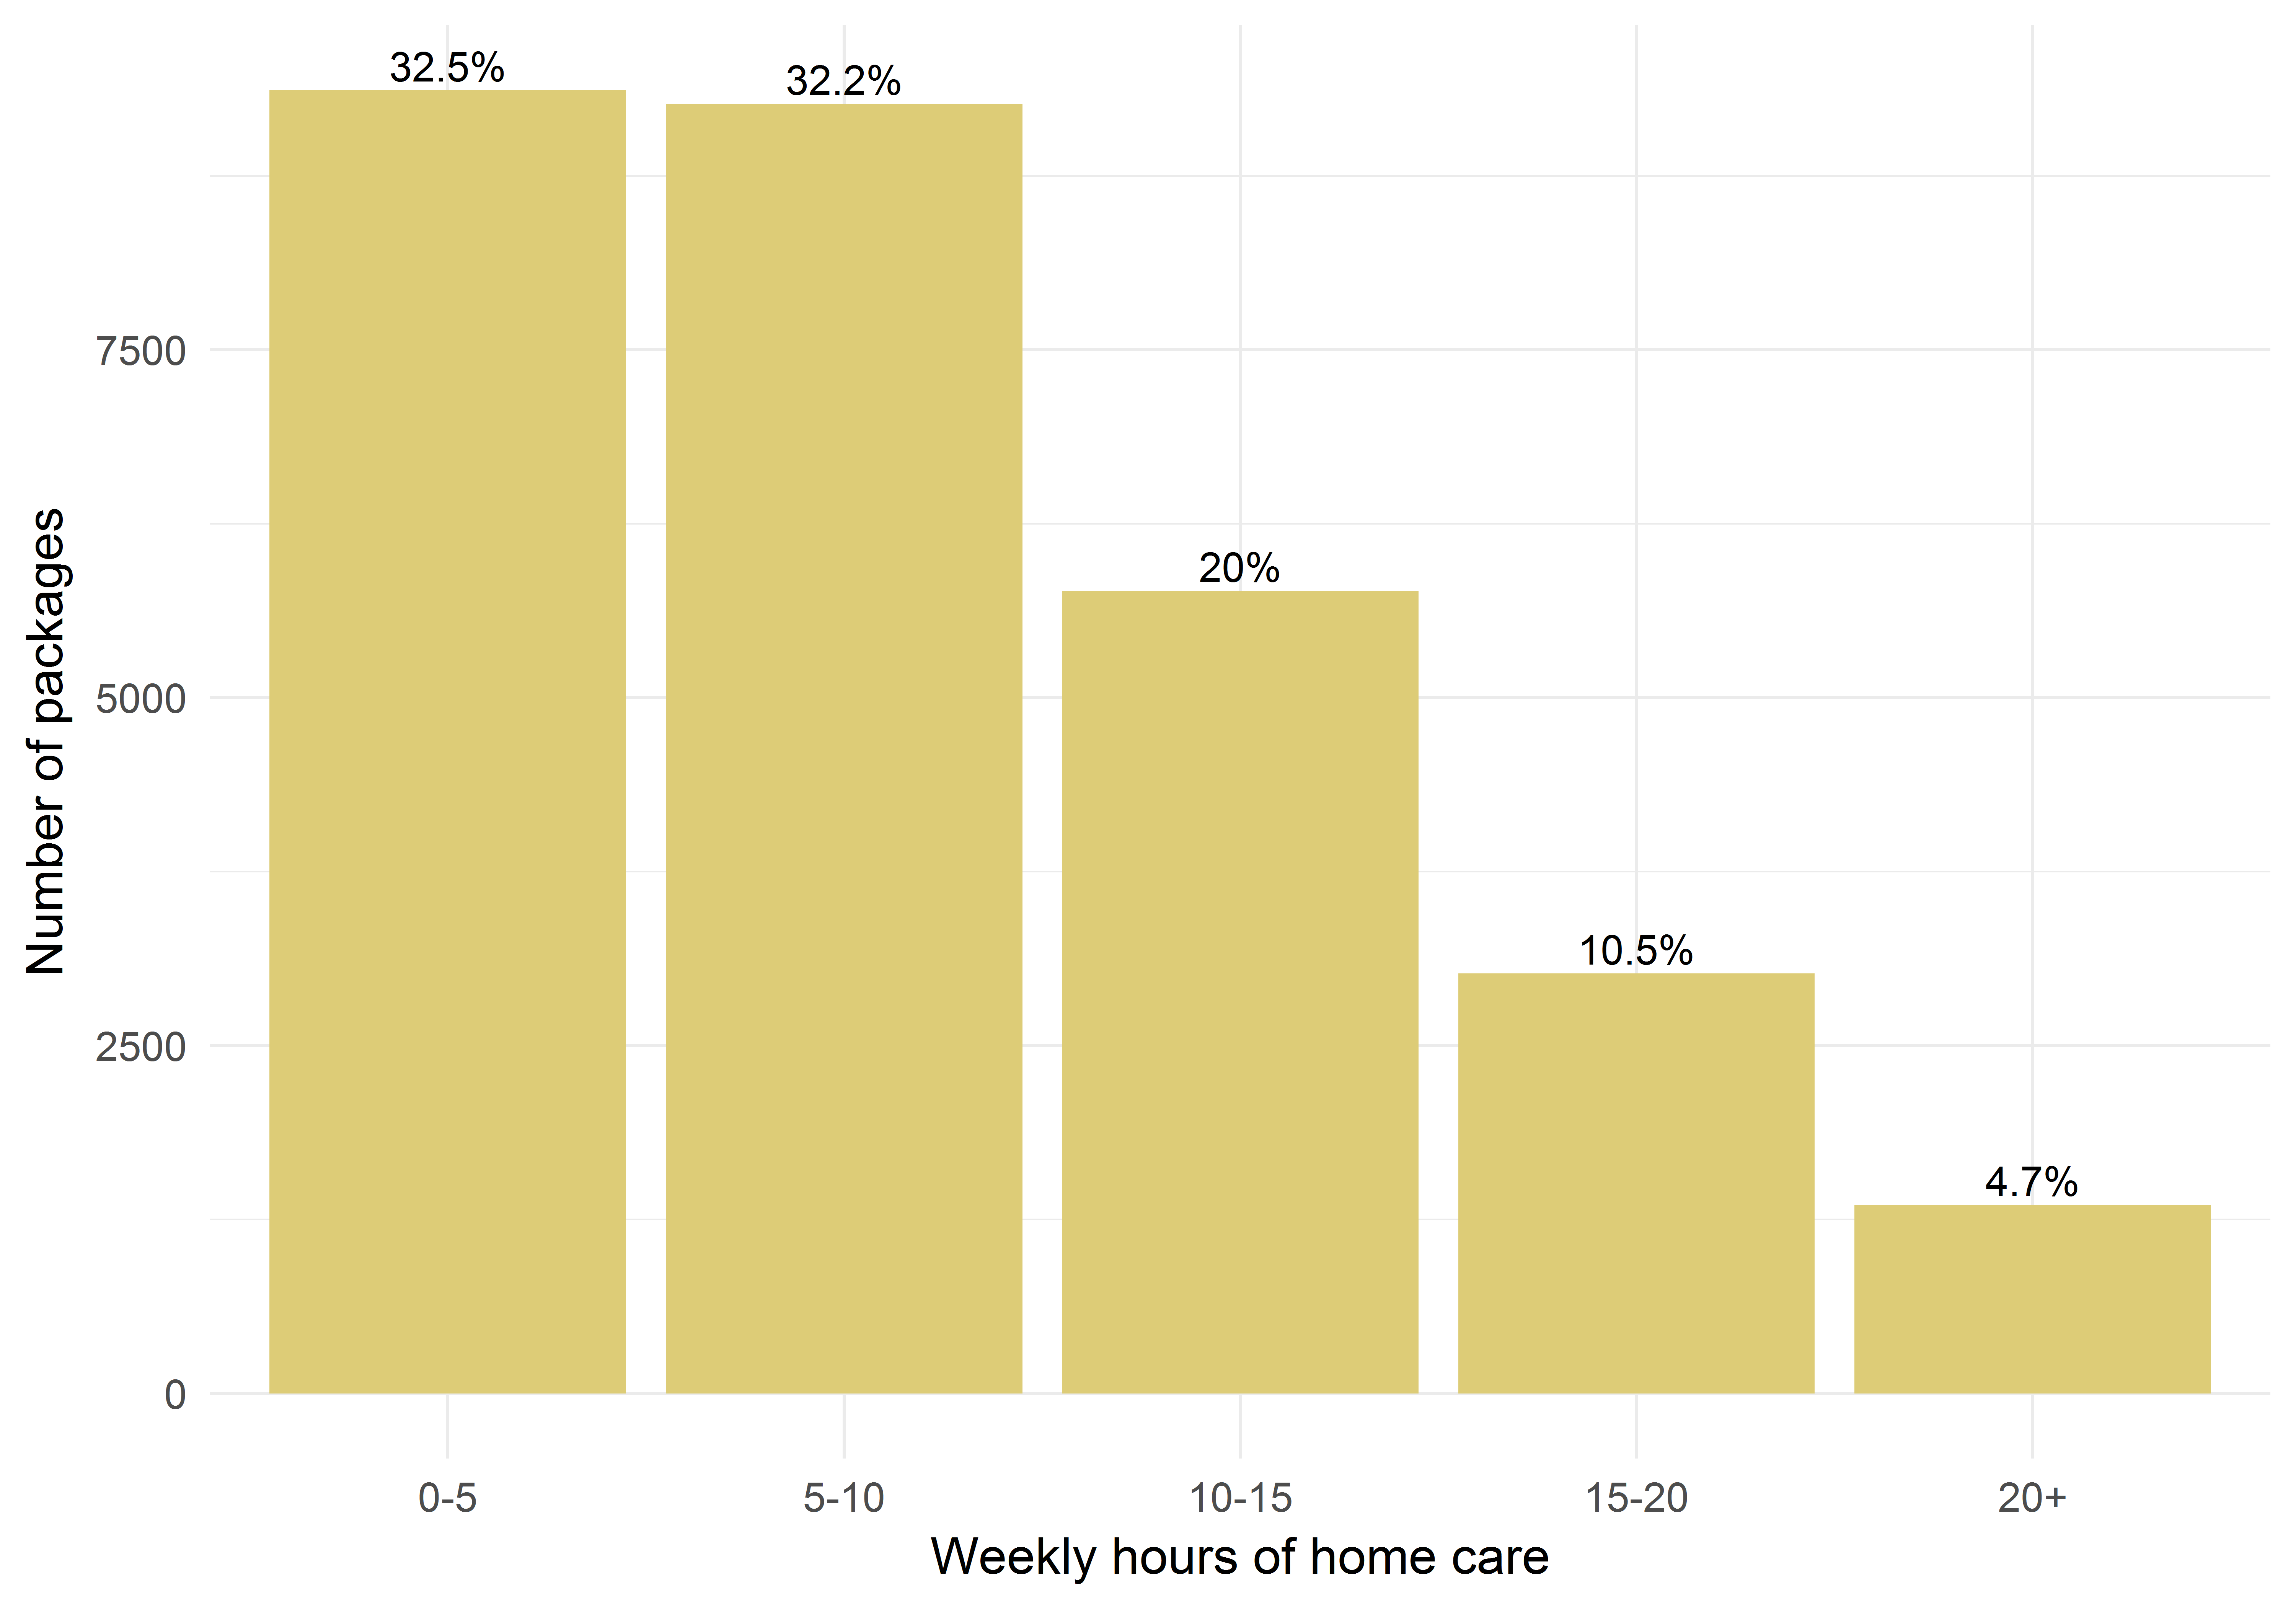
\includegraphics[height = 10cm, width = 12cm]{figures/chapter-renf/04-hrs-plot-ts-subset.png}
    \label{fig:ren-hrs}
\end{figure}

\begin{figure}[]
  \centering
    \caption{Count of packages of care by duration}
    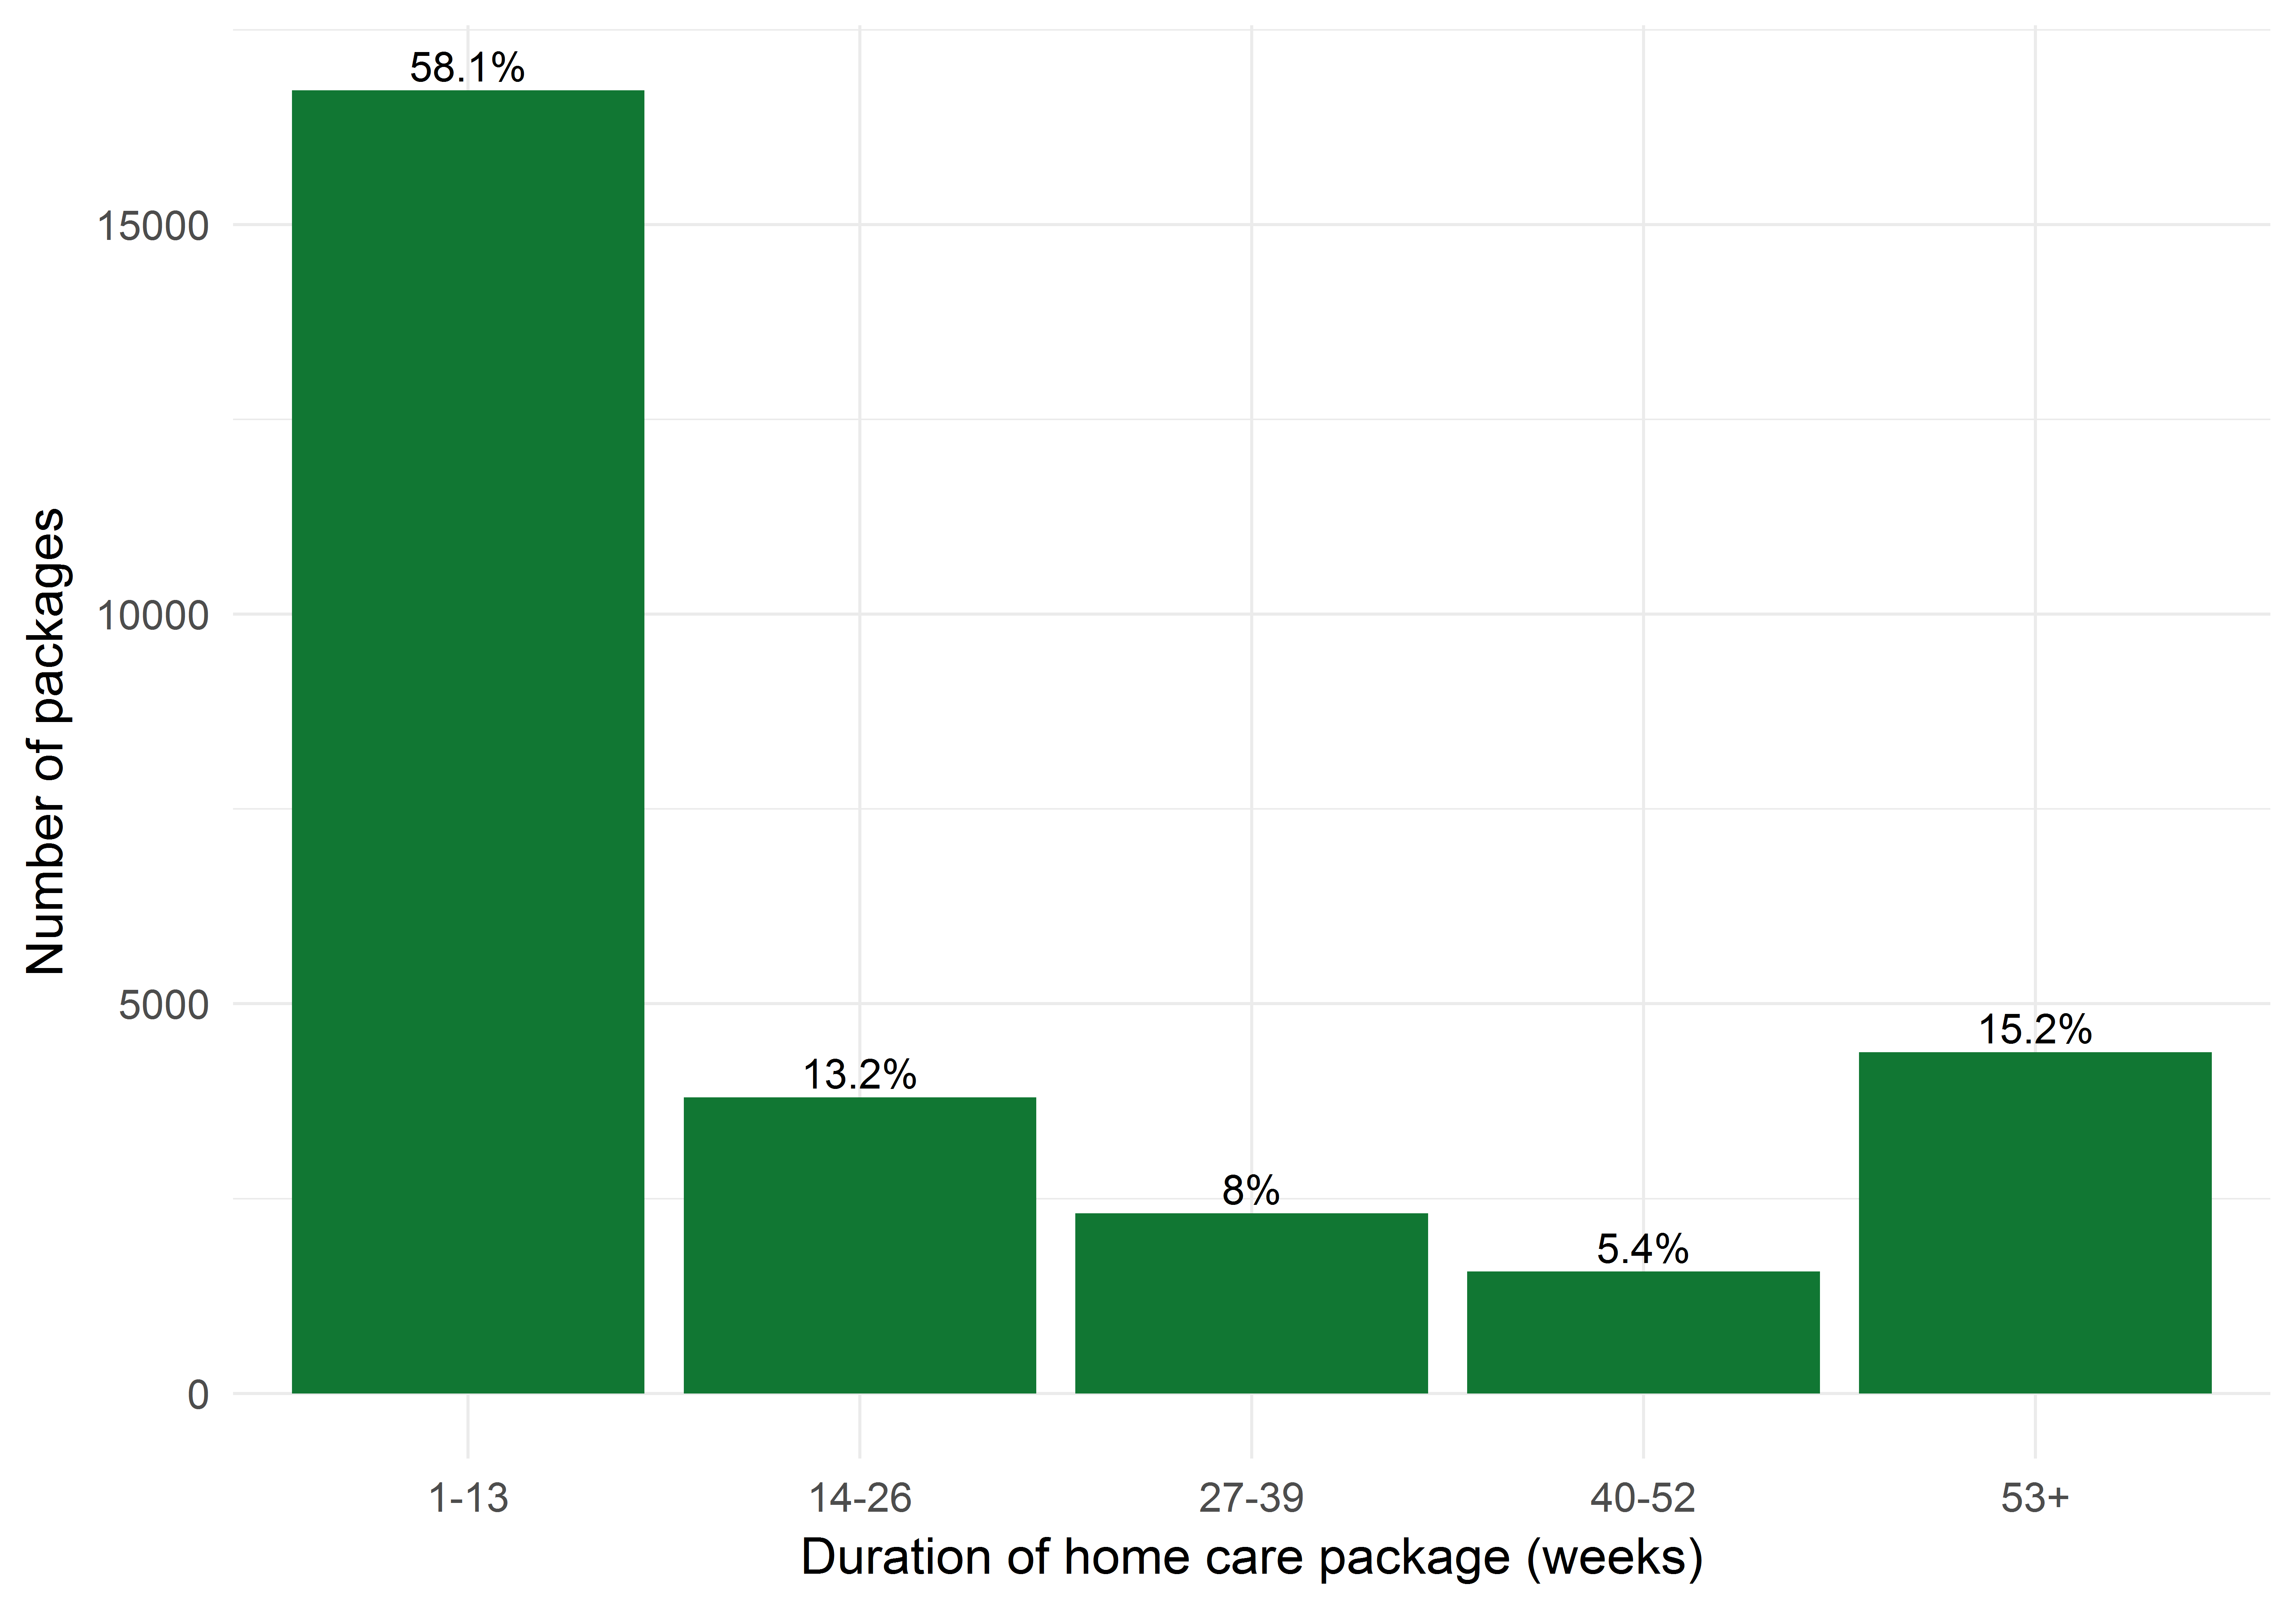
\includegraphics[height = 10cm, width = 12cm]{figures/chapter-renf/05-duration-plot.png}
    \label{fig:ren-duration}
\end{figure}

\FloatBarrier

\subsection{Distribution of individuals receiving home care}\label{renf-results-ts}

Table \ref{tab:renf-ts-summary} and figure \ref{fig:renf-hrs} show the
variation in the number of people receiving home care during each
financial year. There is little weekly variation within years with the
exception of financial year 2010/11 which saw a large drop in the total
number of individuals receiving care. The variation in years following
this show gradual increases and overall numbers return to pre-2010/11
levels by 2014/15.

\begin{figure}[h]
  \centering
    \caption{Variation in the number of individuals receiving home care}
    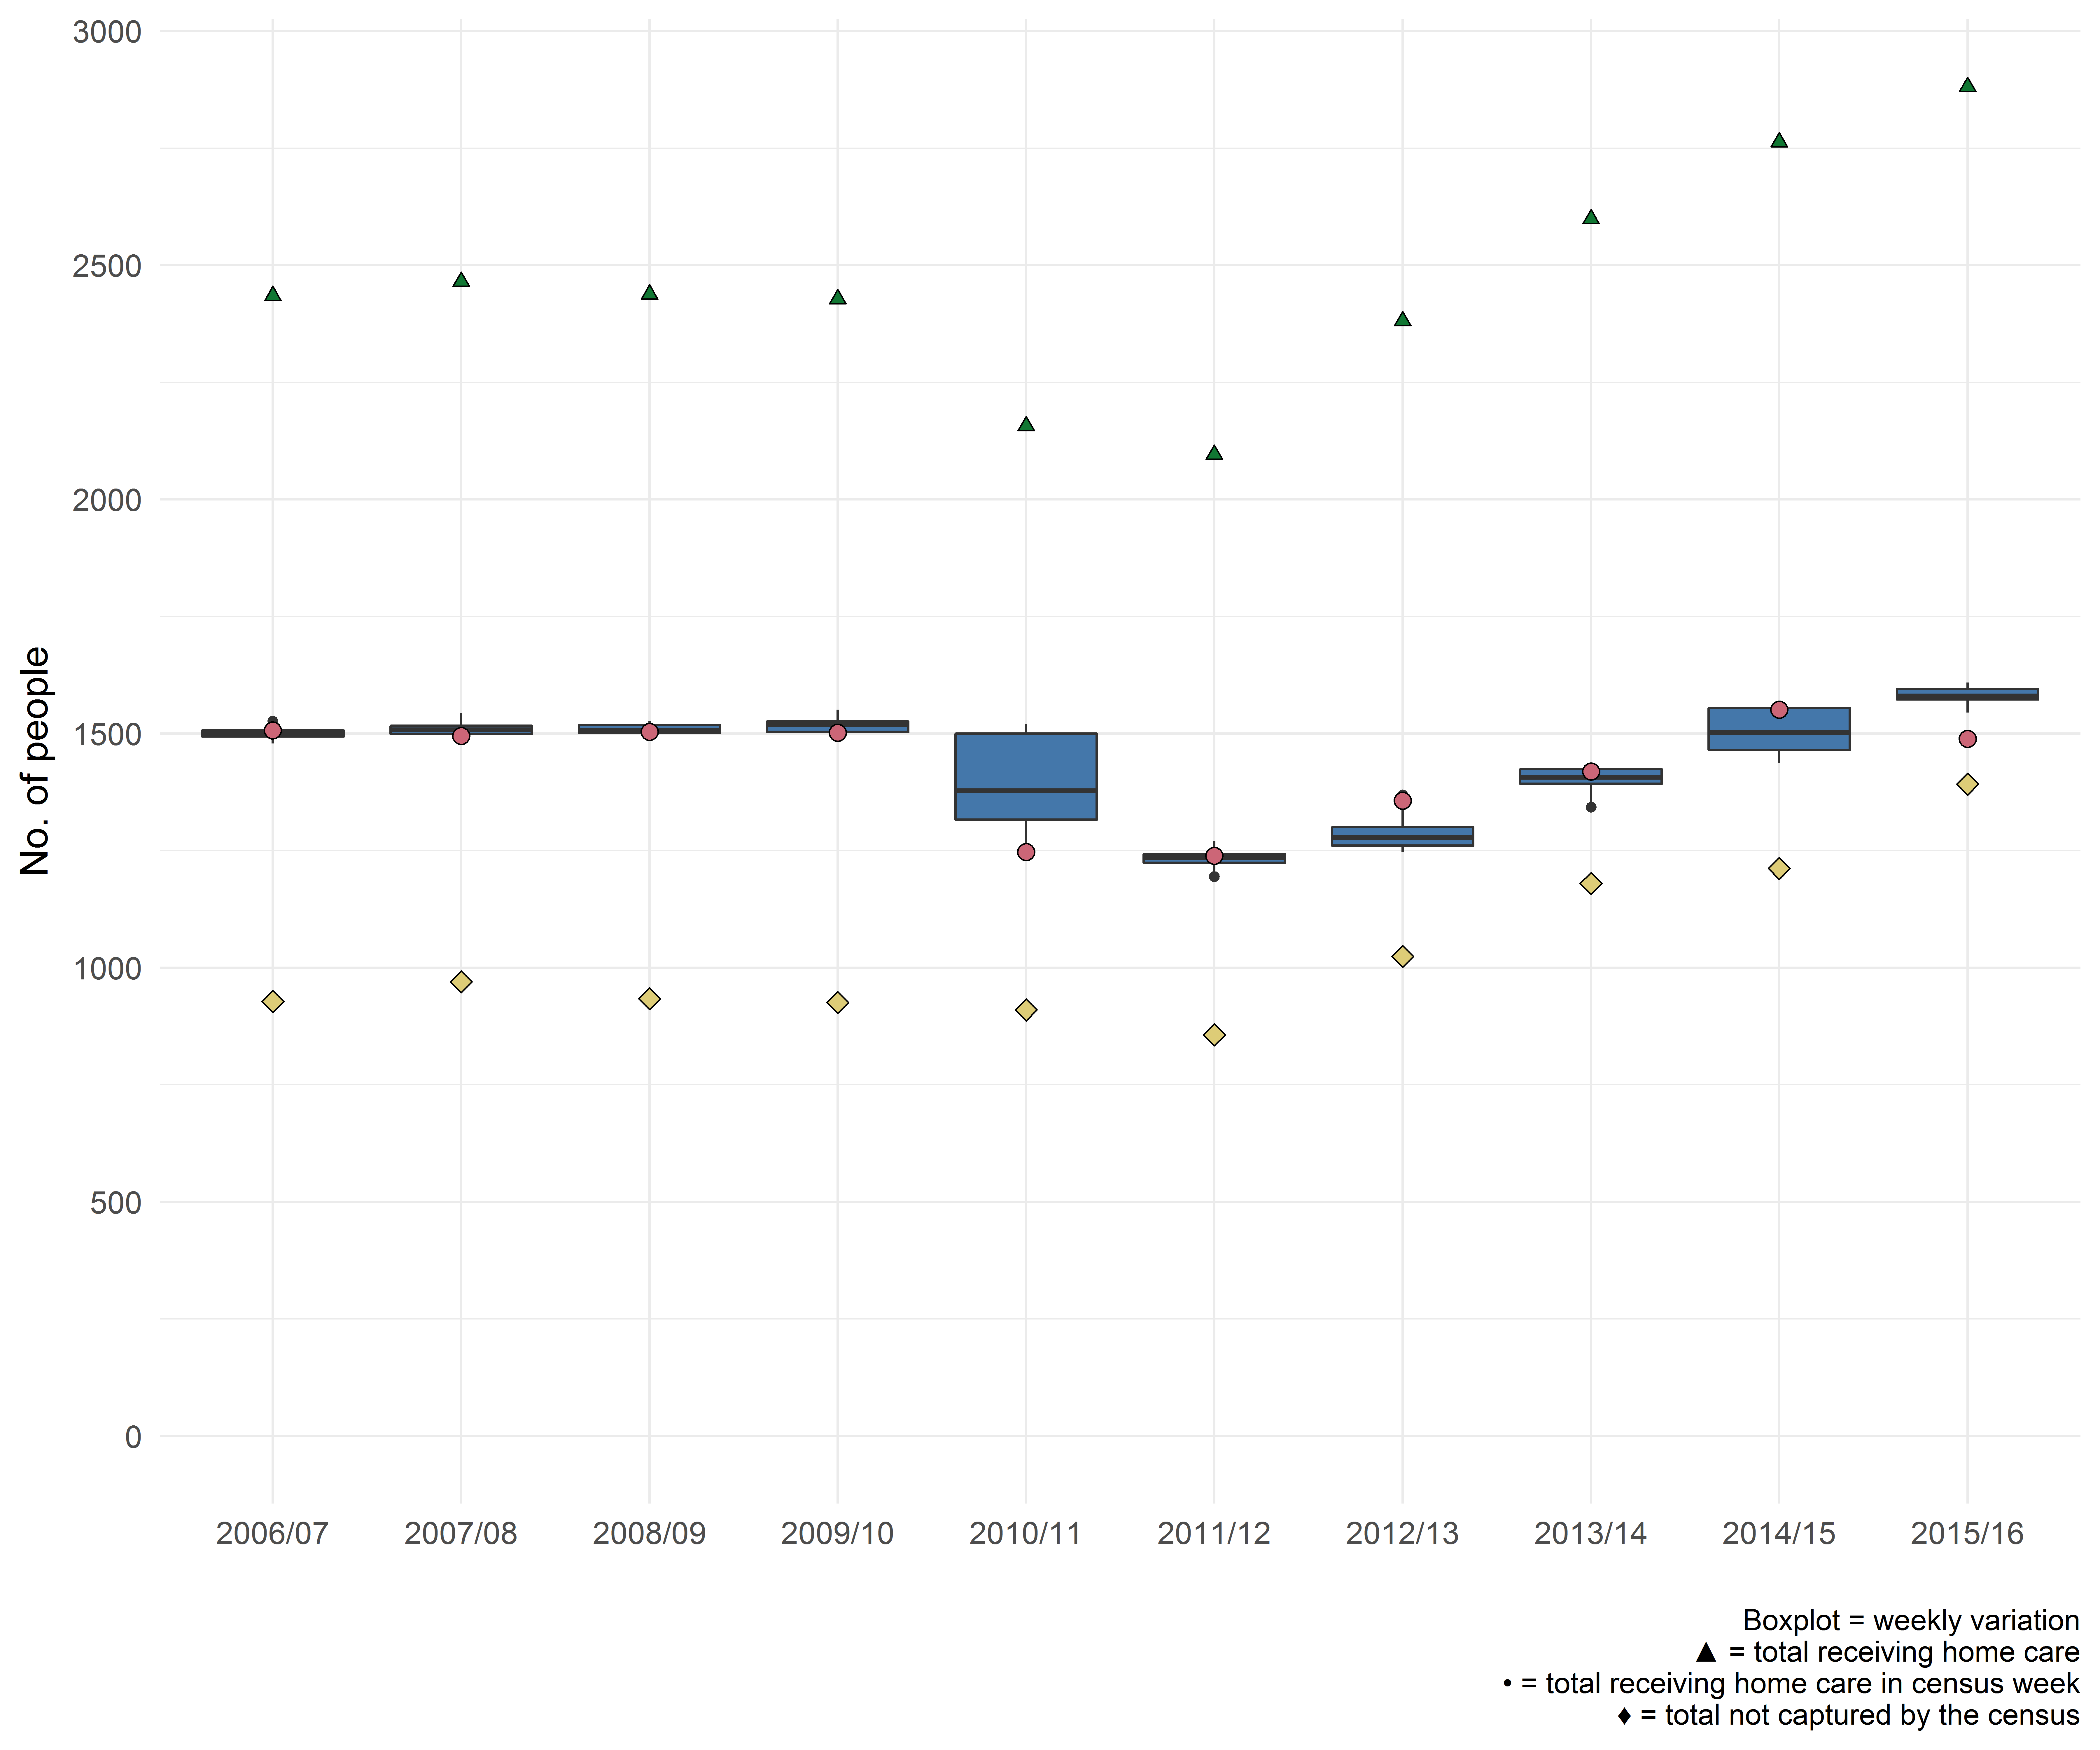
\includegraphics[width = 14cm, height = 22cm]{figures/chapter-renf/06-indivdual-weekly-variation.png}
    \label{fig:renf-hrs}
\end{figure}

Figure \ref{fig:renf-hrs} and table \ref{tab:renf-ts-summary} also
indicate that number of individuals receiving home care and captured by
the census is between 51.7\% and 61.9\% of the total number of
individuals that will receive care in that year. The trend shows a
decreasing proportion of individuals are captured by the census.

\begin{table}[]
\centering
\caption{Variation in the number of individuals receiving home care}
\label{tab:renf-ts-summary}
\resizebox{\textwidth}{!}{%
\begin{tabular}{@{}lrrrrrrrrrr@{}}
\toprule
\textbf{\begin{tabular}[c]{@{}l@{}}Financial\\ Year\end{tabular}} & \textbf{min} & \textbf{max} & \textbf{mean} & \textbf{sd} & \textbf{median} & \textbf{range} & \textbf{IQR} & \textbf{\begin{tabular}[c]{@{}r@{}}Total individuals\\ receiving home\\ care\end{tabular}} & \textbf{\begin{tabular}[c]{@{}r@{}}Total individulas\\ not captured by\\ census\end{tabular}} & \textbf{\begin{tabular}[c]{@{}r@{}}Ratio of individuals\\ captured by census\\ (\%)\end{tabular}} \\ \midrule
\textbf{2006/07} & 1479 & 1527 & 1502.51 & 11.75 & 1501 & 48 & 15 & 2435 & 928 & 61.89 \\
\textbf{2007/08} & 1488 & 1544 & 1508.65 & 12.61 & 1508 & 56 & 18 & 2465 & 970 & 60.65 \\
\textbf{2008/09} & 1486 & 1527 & 1508.63 & 9.96 & 1508 & 41 & 16 & 2438 & 934 & 61.69 \\
\textbf{2009/10} & 1488 & 1551 & 1516.43 & 15.62 & 1520 & 63 & 24 & 2428 & 926 & 61.86 \\
\textbf{2010/11} & 1256 & 1520 & 1399.39 & 90.85 & 1378 & 264 & 176 & 2157 & 910 & 57.81 \\
\textbf{2011/12} & 1195 & 1271 & 1234.19 & 15.21 & 1236 & 76 & 19 & 2096 & 857 & 59.11 \\
\textbf{2012/13} & 1248 & 1369 & 1288.44 & 36.55 & 1278 & 121 & 39 & 2381 & 1024 & 56.99 \\
\textbf{2013/14} & 1343 & 1436 & 1405.52 & 21.17 & 1408 & 93 & 31 & 2599 & 1180 & 54.60 \\
\textbf{2014/15} & 1437 & 1568 & 1505.50 & 44.68 & 1502 & 131 & 90 & 2763 & 1212 & 56.13 \\
\textbf{2015/16} & 1545 & 1609 & 1582.60 & 13.27 & 1580 & 64 & 21 & 2881 & 1392 & 51.68 \\ \bottomrule
\end{tabular}%
}
\end{table}

\FloatBarrier
\subsection{Comparison of individuals with/without any packages in the census}\label{subsec:renf-pack-diff}

Figure \ref{fig:renf-prop-plot} shows that there are similar proportions
of indviduals receiving each type of homecare in each financial year
regardless of whether or not they have any packages of care captured by
the census. The figure also shows the increasing proportion of
``Reablement'' packages over time from almost no packages in 2010/11 to
approximately 14\% of all packages delivered in 2014/15. ``Care at home
(Mainstream)'' type packages saw a drop from approximately 82\% to 60\%
of all packages over the same period.

\begin{figure}[h]
  \centering
    \caption{Proportion of individuals receiving home care}
    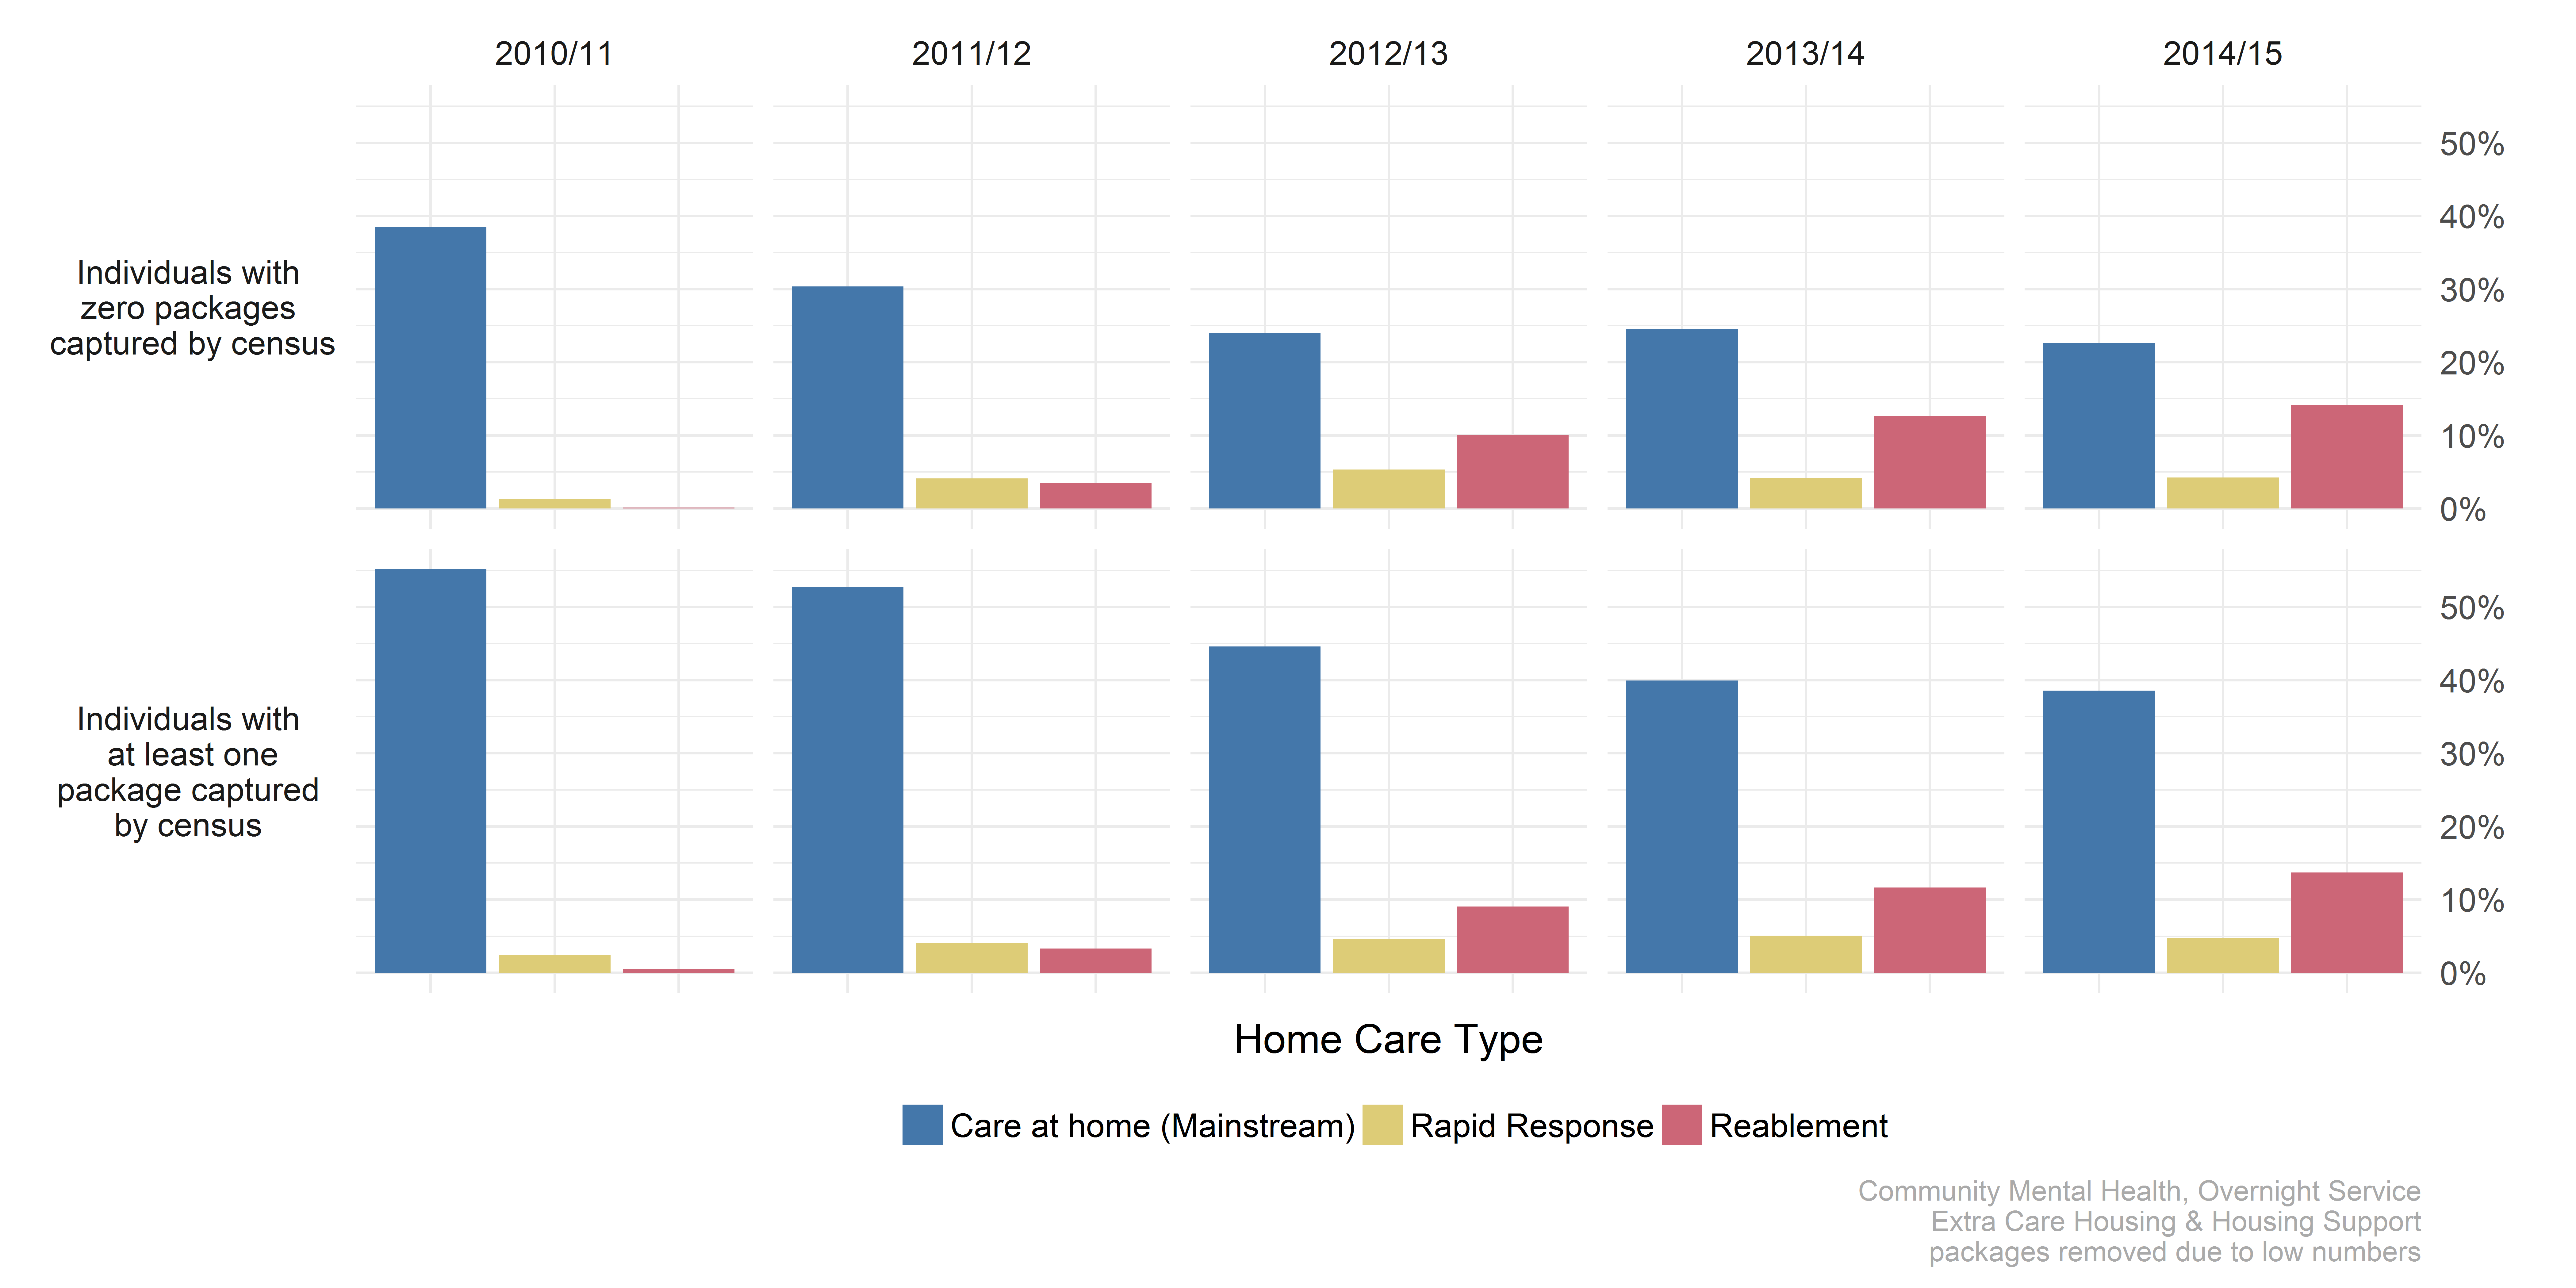
\includegraphics{figures/chapter-renf/12-census-prop-plot.png}
    \label{fig:renf-prop-plot}
\end{figure}

\subsection{Comparison of package intensity for indiviudals with/without any packages in the census}\label{subsec:renf-inten-diff}

Comparison of the total weekly hours of home care (intensity) that
indivduals with/without any packages in the census receive (figure
\ref{fig:renf-inten}) shows that there is very little difference in
median values. However, as time progresses, the median value for total
hours of home care is slightly larger for those with no packages of care
captured in the census.

This trend is shown in table \ref{tab:renf-regr-inten} which shows the
intercept and coefficient of total hours of home care in linear
regression models for each year (in bold) with presence of at least one,
or zero packages in the census as a categorical predictor. Over time,
the intercept value increases from 6.26 hours in 2010/11 to 8.41 hrs in
2014/15 indicating a general increase in intensity for individuals with
at least one package in the census. There is a statistically significant
difference in the amount of hours of care received betweeen those that
have at lease one package in the census and those that have no packages
in every financial year. The coefficient value is negatice in 2010/11
but positive in all other years and increases over time. However, the
difference in groups is modest (the 1.2 hrs increase in intensity in
2014/15 is equivalent to approximately 10 minutes extra care per day).

\begin{figure}[h]
  \centering
    \caption{Variation in intensity of home care}
    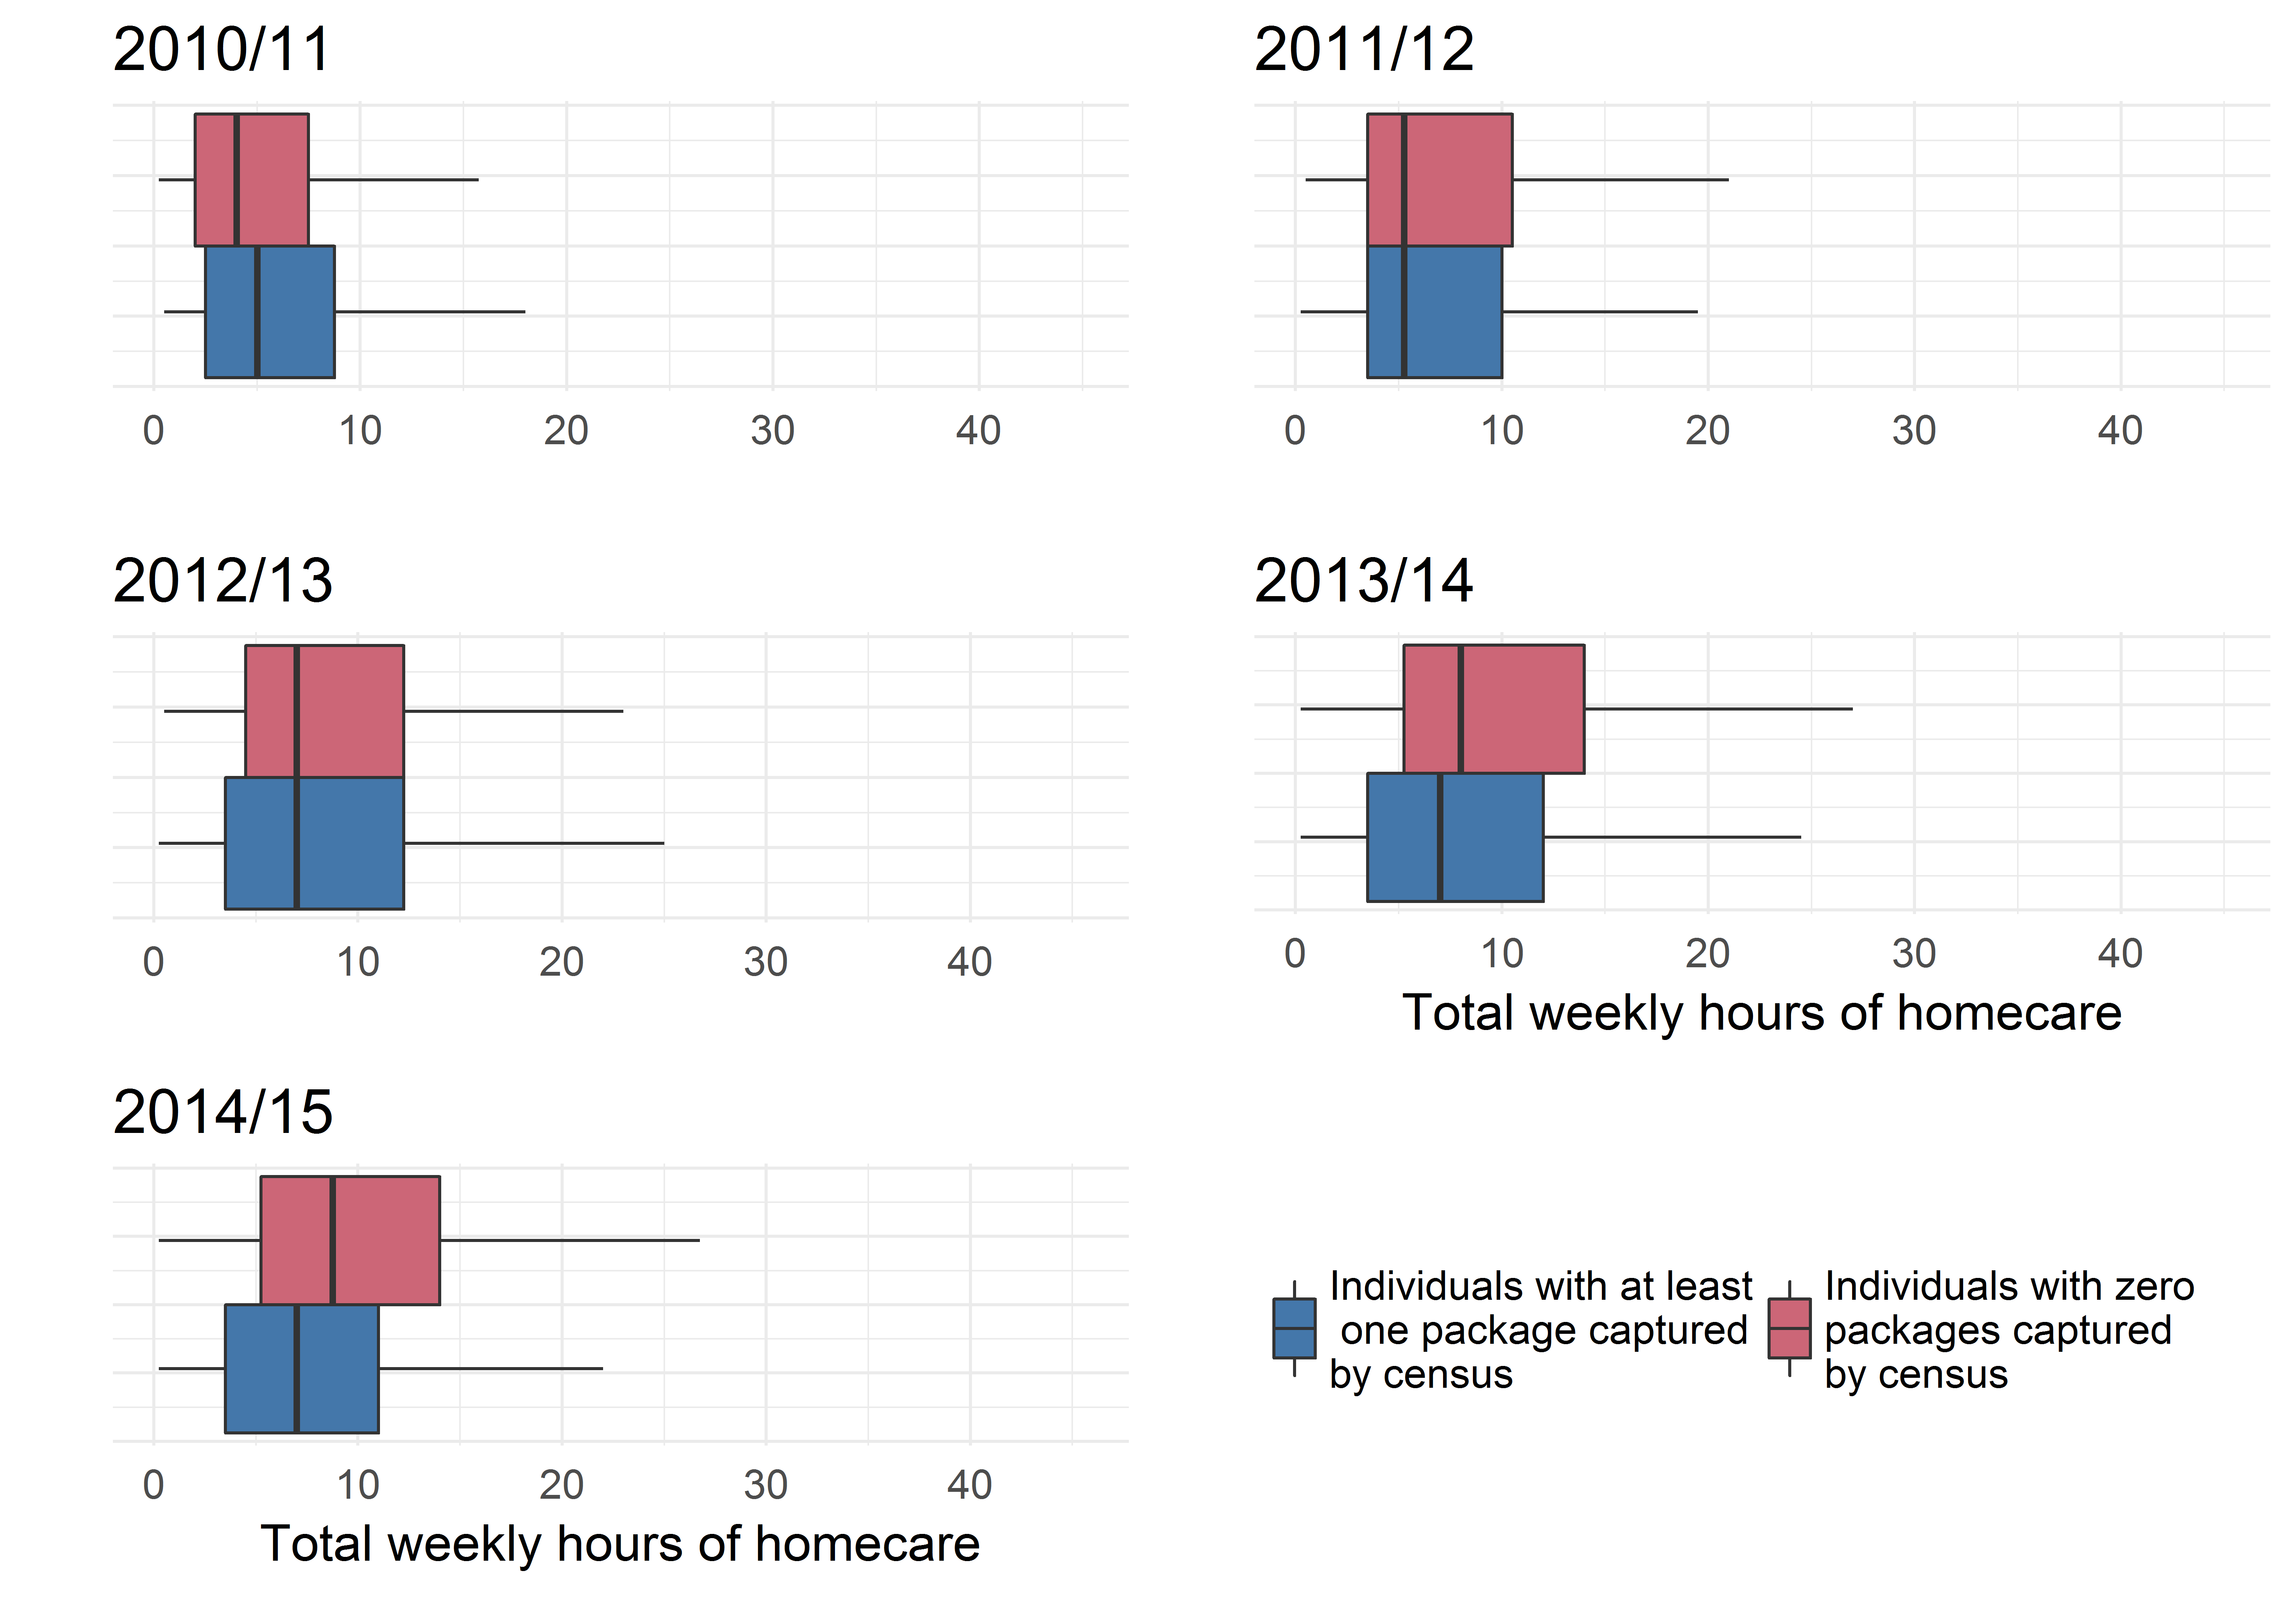
\includegraphics{figures/chapter-renf/14-inten.png}
    \label{fig:renf-inten}
\end{figure}

Table \ref{tab:renf-regr-inten} also shows the results of the same
linear regression model applied seperately to individuals from groups of
different gender, age, and home care type. The differences between
theses groups become more apparent over time with all groups (apart from
the ``Rapid Response'' care type) showing statistically significant
differences in 2014/15. Intercept values for total hours of home care
vary slightly across different groups with ``Rapid Response'' and
``Reablement'' packages more likely to have higher values - particularly
in later years. Differences between groups also vary with older age
groups and ``Reablement'' care type packages showing larger coefficient
values for those with zero packages captured by the census. The largest
difference is seen for ``Reablement'' packages in 2014/15 with an
expected 2.14 hrs increase for those with zero packages compared to
those with at least one package in the census. This is equivalent to an
18.3 minute increase in care per day. The variation in total hours of
care between home care types is plotted in figure
\ref{fig:renf-intensity-type}.

\begin{landscape}
\begin{longtable}[c]{@{}lllllllll@{}}
\caption{Regression models of package intensity}
\label{tab:renf-regr-inten}\\
\toprule
\textbf{\begin{tabular}[c]{@{}l@{}}Financial\\ Year\end{tabular}} & \textbf{Gender} & \textbf{Age group} & \textbf{Type of home care} & \textbf{} & \textbf{estimate} & \textbf{std.error} & \textbf{statistic} & \textbf{p value} \\* \midrule
\endfirsthead
%
\multicolumn{9}{c}%
{{\bfseries Table \thetable\ continued from previous page}} \\
\toprule
\textbf{\begin{tabular}[c]{@{}l@{}}Financial\\ Year\end{tabular}} & \textbf{Gender} & \textbf{Age group} & \textbf{Type of home care} & \textbf{} & \textbf{estimate} & \textbf{std.error} & \textbf{statistic} & \textbf{p value} \\* \midrule
\endhead
%
\bottomrule
\endfoot
%
\endlastfoot
%
\textbf{2010/11} & \textbf{} & \textbf{} & \textbf{} & \textbf{(Intercept)} & \textbf{6.255} & \textbf{0.115} & \textbf{54.630} & \textbf{} \\
\textbf{} & \textbf{} & \textbf{} & \textbf{} & \textbf{No package in census} & \textbf{-0.415} & \textbf{0.193} & \textbf{-2.147} & \textbf{\textless{}0.05} \\
 & Female &  &  & (Intercept) & 6.184 & 0.134 & 46.091 &  \\
 & Female &  &  & No package in census & -0.435 & 0.234 & -1.861 & 0.063 \\
 & Male &  &  & (Intercept) & 6.450 & 0.220 & 29.338 &  \\
 & Male &  &  & No package in census & -0.428 & 0.346 & -1.237 & 0.217 \\
 &  & 65-75 &  & (Intercept) & 7.200 & 0.243 & 29.573 &  \\
 &  & 65-75 &  & No package in census & -1.534 & 0.417 & -3.678 & \textless{}0.05 \\
 &  & 76-85 &  & (Intercept) & 5.803 & 0.164 & 35.386 &  \\
 &  & 76-85 &  & No package in census & -0.084 & 0.276 & -0.303 & 0.762 \\
 &  & 86 plus &  & (Intercept) & 6.065 & 0.204 & 29.764 &  \\
 &  & 86 plus &  & No package in census & 0.119 & 0.340 & 0.349 & 0.727 \\
 &  &  & Care at home (Mainstream) & (Intercept) & 6.266 & 0.118 & 53.245 &  \\
 &  &  & Care at home (Mainstream) & No package in census & -0.430 & 0.198 & -2.177 & \textless{}0.05 \\
 &  &  & Rapid Response & (Intercept) & 5.470 & 0.490 & 11.169 &  \\
 &  &  & Rapid Response & No package in census & 0.332 & 0.908 & 0.365 & 0.716 \\
 &  &  & Reablement & (Intercept) & 9.958 & 1.602 & 6.216 &  \\
 &  &  & Reablement & No package in census & -1.792 & 3.582 & -0.500 & 0.625 \\
 \\
 \\
 \\
\textbf{2011/12} & \textbf{} & \textbf{} & \textbf{} & \textbf{(Intercept)} & \textbf{6.754} & \textbf{0.118} & \textbf{57.119} & \textbf{} \\
\textbf{} & \textbf{} & \textbf{} & \textbf{} & \textbf{No package in census} & \textbf{0.426} & \textbf{0.203} & \textbf{2.097} & \textbf{\textless{}0.05} \\
 & Female &  &  & (Intercept) & 6.701 & 0.146 & 46.012 &  \\
 & Female &  &  & No package in census & 0.485 & 0.251 & 1.929 & 0.054 \\
 & Male &  &  & (Intercept) & 6.871 & 0.201 & 34.101 &  \\
 & Male &  &  & No package in census & 0.297 & 0.344 & 0.866 & 0.387 \\
 &  & 65-75 &  & (Intercept) & 7.414 & 0.224 & 33.119 &  \\
 &  & 65-75 &  & No package in census & -0.504 & 0.434 & -1.161 & 0.246 \\
 &  & 76-85 &  & (Intercept) & 6.391 & 0.175 & 36.605 &  \\
 &  & 76-85 &  & No package in census & 0.718 & 0.291 & 2.468 & \textless{}0.05 \\
 &  & 86 plus &  & (Intercept) & 6.576 & 0.229 & 28.772 &  \\
 &  & 86 plus &  & No package in census & 0.892 & 0.373 & 2.390 & \textless{}0.05 \\
 &  &  & Care at home (Mainstream) & (Intercept) & 6.551 & 0.127 & 51.631 &  \\
 &  &  & Care at home (Mainstream) & No package in census & 0.295 & 0.223 & 1.323 & 0.186 \\
 &  &  & Rapid Response & (Intercept) & 7.770 & 0.413 & 18.826 &  \\
 &  &  & Rapid Response & No package in census & 0.748 & 0.634 & 1.180 & 0.239 \\
 &  &  & Reablement & (Intercept) & 8.573 & 0.480 & 17.868 &  \\
 &  &  & Reablement & No package in census & 0.250 & 0.737 & 0.339 & 0.735 \\
 \\
 \\
 \\
\textbf{2012/13} & \textbf{} & \textbf{} & \textbf{} & \textbf{(Intercept)} & \textbf{8.375} & \textbf{0.118} & \textbf{70.736} & \textbf{} \\
\textbf{} & \textbf{} & \textbf{} & \textbf{} & \textbf{No package in census} & \textbf{0.586} & \textbf{0.202} & \textbf{2.896} & \textbf{\textless{}0.05} \\
 & Female &  &  & (Intercept) & 8.460 & 0.144 & 58.950 &  \\
 & Female &  &  & No package in census & 0.363 & 0.249 & 1.458 & 0.145 \\
 & Male &  &  & (Intercept) & 8.190 & 0.209 & 39.100 &  \\
 & Male &  &  & No package in census & 1.031 & 0.348 & 2.964 & \textless{}0.05 \\
 &  & 65-75 &  & (Intercept) & 8.034 & 0.231 & 34.830 &  \\
 &  & 65-75 &  & No package in census & 0.917 & 0.383 & 2.394 & \textless{}0.05 \\
 &  & 76-85 &  & (Intercept) & 8.398 & 0.181 & 46.311 &  \\
 &  & 76-85 &  & No package in census & 0.544 & 0.306 & 1.779 & \textless{}0.05 \\
 &  & 86 plus &  & (Intercept) & 8.611 & 0.212 & 40.545 &  \\
 &  & 86 plus &  & No package in census & 0.391 & 0.381 & 1.027 & 0.304 \\
 &  &  & Care at home (Mainstream) & (Intercept) & 8.054 & 0.140 & 57.715 &  \\
 &  &  & Care at home (Mainstream) & No package in census & 0.139 & 0.248 & 0.561 & 0.575 \\
 &  &  & Rapid Response & (Intercept) & 10.172 & 0.388 & 26.193 &  \\
 &  &  & Rapid Response & No package in census & -0.218 & 0.589 & -0.370 & 0.712 \\
 &  &  & Reablement & (Intercept) & 8.830 & 0.262 & 33.668 &  \\
 &  &  & Reablement & No package in census & 1.806 & 0.419 & 4.309 & \textless{}0.05 \\
 \\
 \\
 \\
\textbf{2013/14} & \textbf{} & \textbf{} & \textbf{} & \textbf{(Intercept)} & \textbf{8.531} & \textbf{0.117} & \textbf{72.894} & \textbf{} \\
\textbf{} & \textbf{} & \textbf{} & \textbf{} & \textbf{No package in census} & \textbf{0.995} & \textbf{0.198} & \textbf{5.038} & \textbf{\textless{}0.05} \\
 & Female &  &  & (Intercept) & 8.560 & 0.145 & 58.926 &  \\
 & Female &  &  & No package in census & 1.092 & 0.253 & 4.322 & \textless{}0.05 \\
 & Male &  &  & (Intercept) & 8.464 & 0.196 & 43.167 &  \\
 & Male &  &  & No package in census & 0.844 & 0.313 & 2.699 & \textless{}0.05 \\
 &  & 65-75 &  & (Intercept) & 8.624 & 0.222 & 38.794 &  \\
 &  & 65-75 &  & No package in census & 0.774 & 0.387 & 2.001 & \textless{}0.05 \\
 &  & 76-85 &  & (Intercept) & 8.420 & 0.176 & 47.958 &  \\
 &  & 76-85 &  & No package in census & 0.953 & 0.295 & 3.233 & \textless{}0.05 \\
 &  & 86 plus &  & (Intercept) & 8.607 & 0.221 & 38.879 &  \\
 &  & 86 plus &  & No package in census & 1.240 & 0.367 & 3.378 & \textless{}0.05 \\
 &  &  & Care at home (Mainstream) & (Intercept) & 8.159 & 0.143 & 57.052 &  \\
 &  &  & Care at home (Mainstream) & No package in census & 0.766 & 0.247 & 3.101 & \textless{}0.05 \\
 &  &  & Rapid Response & (Intercept) & 9.621 & 0.356 & 27.037 &  \\
 &  &  & Rapid Response & No package in census & 0.944 & 0.603 & 1.565 & 0.118 \\
 &  &  & Reablement & (Intercept) & 9.239 & 0.241 & 38.259 &  \\
 &  &  & Reablement & No package in census & 1.364 & 0.383 & 3.562 & \textless{}0.05 \\
 \\
 \\
 \\
\textbf{2014/15} & \textbf{} & \textbf{} & \textbf{} & \textbf{(Intercept)} & \textbf{8.411} & \textbf{0.114} & \textbf{73.466} & \textbf{} \\
\textbf{} & \textbf{} & \textbf{} & \textbf{} & \textbf{No package in census} & \textbf{1.197} & \textbf{0.189} & \textbf{6.340} & \textbf{\textless{}0.05} \\
 & Female &  &  & (Intercept) & 8.369 & 0.141 & 59.267 &  \\
 & Female &  &  & No package in census & 1.298 & 0.234 & 5.539 & \textless{}0.05 \\
 & Male &  &  & (Intercept) & 8.498 & 0.195 & 43.498 &  \\
 & Male &  &  & No package in census & 0.996 & 0.319 & 3.126 & \textless{}0.05 \\
 &  & 65-75 &  & (Intercept) & 8.427 & 0.219 & 38.538 &  \\
 &  & 65-75 &  & No package in census & 0.878 & 0.383 & 2.294 & \textless{}0.05 \\
 &  & 76-85 &  & (Intercept) & 8.374 & 0.169 & 49.619 &  \\
 &  & 76-85 &  & No package in census & 1.175 & 0.280 & 4.201 & \textless{}0.05 \\
 &  & 86 plus &  & (Intercept) & 8.458 & 0.222 & 38.051 &  \\
 &  & 86 plus &  & No package in census & 1.456 & 0.347 & 4.194 & \textless{}0.05 \\
 &  &  & Care at home (Mainstream) & (Intercept) & 8.004 & 0.138 & 57.848 &  \\
 &  &  & Care at home (Mainstream) & No package in census & 0.623 & 0.238 & 2.617 & \textless{}0.05 \\
 &  &  & Rapid Response & (Intercept) & 9.992 & 0.385 & 25.960 &  \\
 &  &  & Rapid Response & No package in census & 0.694 & 0.612 & 1.134 & 0.257 \\
 &  &  & Reablement & (Intercept) & 8.898 & 0.230 & 38.757 &  \\
 &  &  & Reablement & No package in census & 2.135 & 0.352 & 6.072 & \textless{}0.05 \\* \bottomrule
\end{longtable}
\end{landscape}

\begin{figure}[]
  \centering
    \caption{Variation in intensity of home care - by type}
    \includegraphics{figures/chapter-renf/16-type-inten.png}
    \label{fig:renf-intensity-type}
\end{figure}

\FloatBarrier
\subsection{Comparison of package duration for indiviudals with/without any packages in the census}\label{subsec:renf-duration-diff}

Figure \ref{fig:renf-duration} shows a comparison of the total duration
of care for indiviudals with or without any packages in the census for
each financial year. A clear difference can be seen for those with no
packages captured by the census who have much shorter total duration of
care. Results of linear regression models plotting package duration
against presence or not of at least one package in the census (table
\ref{tab:renf-regr-duration}) confirms statistically significant
differences between all groups (with the exception of ``Reablement''
packages in 2010/11). These differences are large e.g.~the overall
coefficient in 2014/14 is -54.32 weeks suggesting individuals with zero
packages captured by the census have care duration, on average, over a
year shorter than those with at least one package in the census.

Intercept values in table \ref{tab:renf-regr-duration} gradually
decrease over time which is likely due to censoring at the end of the
time series. Within years there is a large difference in intercept
values. Older age groups, as well as ``Rapid Response'' and
``Reablement'' type packages all show much lower values than the total
seen in each year. Variation in duration of care by home care type is
plotted in figure \ref{fig:renf-dur-type}

\begin{figure}[h]
  \centering
    \caption{Variation in duration of home care}
    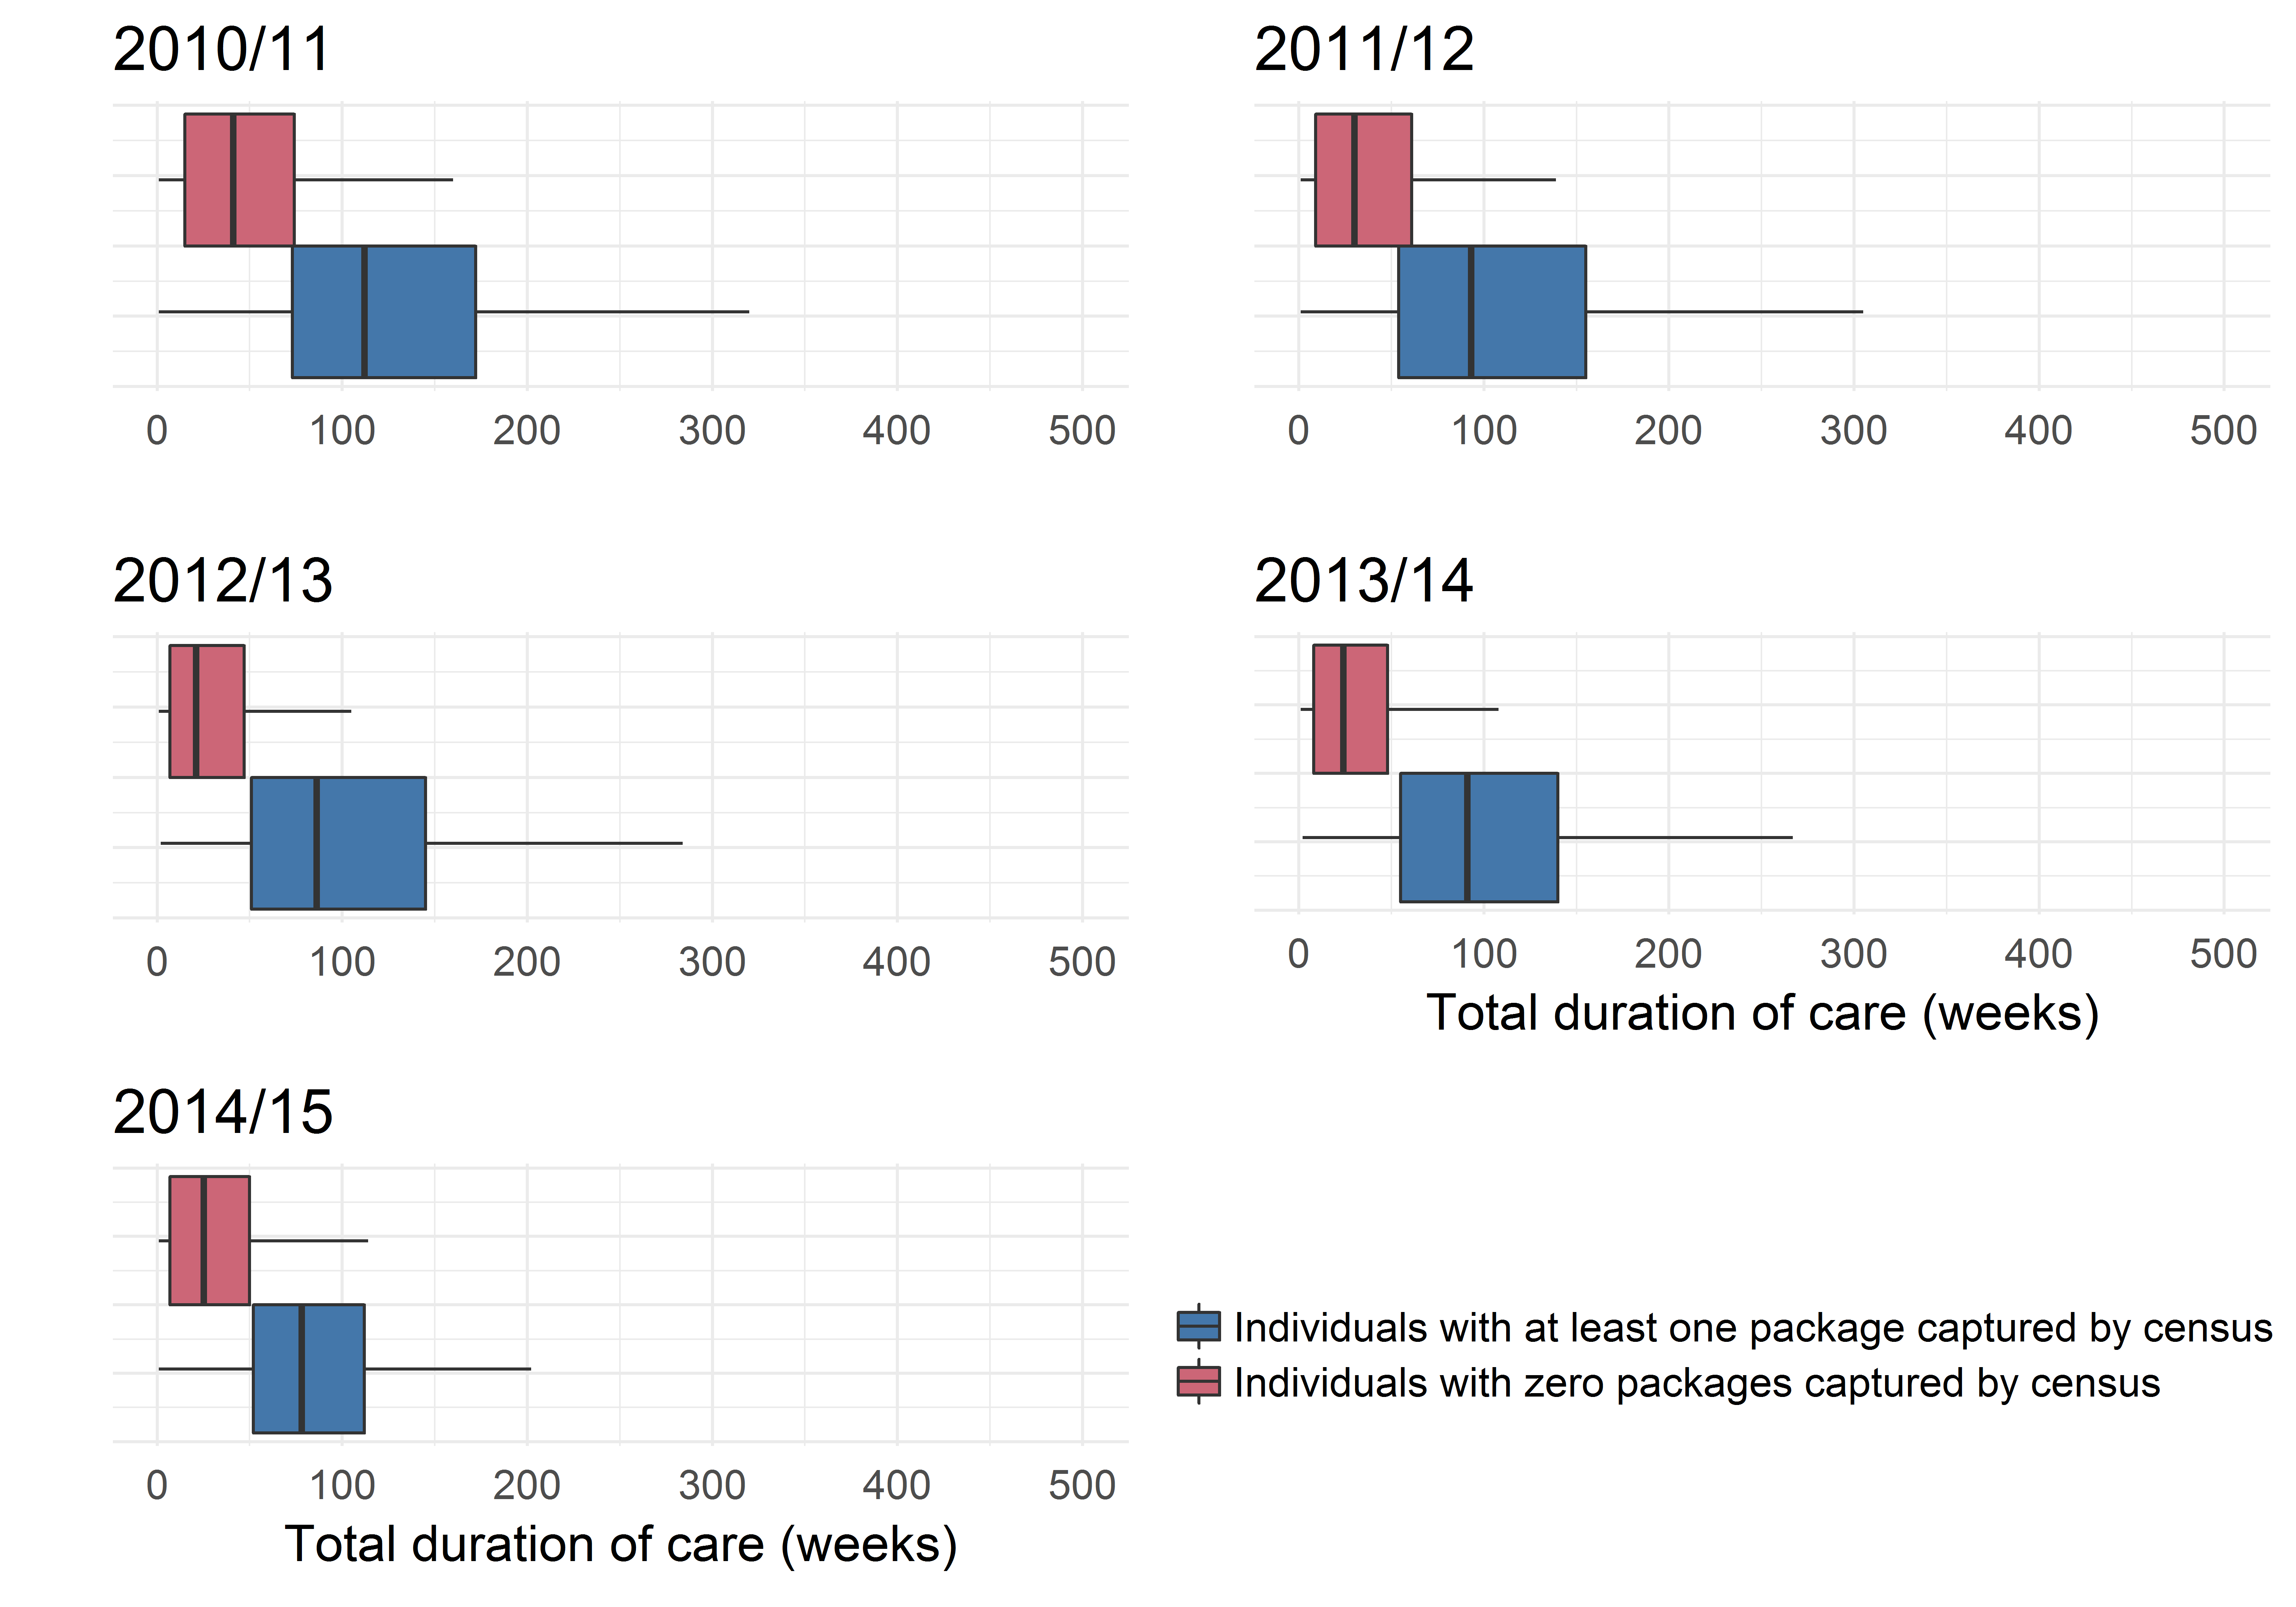
\includegraphics{figures/chapter-renf/17-duration.png}
    \label{fig:renf-duration}
\end{figure}

\begin{landscape}
\begin{longtable}[c]{@{}lllllllll@{}}
\caption{Regression models of package duration}
\label{tab:renf-regr-duration}\\
\toprule
\textbf{\begin{tabular}[c]{@{}l@{}}Financial\\ Year\end{tabular}} & \textbf{Gender} & \textbf{Age group} & \textbf{Type of home care} & \textbf{} & \textbf{estimate} & \textbf{std.error} & \textbf{statistic} & \textbf{p value} \\* \midrule
\endfirsthead
%
\multicolumn{9}{c}%
{{\bfseries Table \thetable\ continued from previous page}} \\
\toprule
\textbf{\begin{tabular}[c]{@{}l@{}}Financial\\ Year\end{tabular}} & \textbf{Gender} & \textbf{Age group} & \textbf{Type of home care} & \textbf{} & \textbf{estimate} & \textbf{std.error} & \textbf{statistic} & \textbf{p value} \\* \midrule
\endhead
%
\bottomrule
\endfoot
%
\endlastfoot
%
\textbf{2010/11} & \textbf{} & \textbf{} & \textbf{} & \textbf{(Intercept)} & \textbf{131.19} & \textbf{1.55} & \textbf{84.80} & \textbf{} \\
\textbf{} & \textbf{} & \textbf{} & \textbf{} & \textbf{No package in census} & \textbf{-76.55} & \textbf{2.62} & \textbf{-29.18} & \textbf{\textless{}0.05} \\
 & Female &  &  & (Intercept) & 132.62 & 1.83 & 72.40 &  \\
 & Female &  &  & No package in census & -75.29 & 3.20 & -23.54 & \textless{}0.05 \\
 & Male &  &  & (Intercept) & 127.36 & 2.89 & 44.12 &  \\
 & Male &  &  & No package in census & -78.09 & 4.59 & -17.01 & \textless{}0.05 \\
 &  & 65-75 &  & (Intercept) & 146.55 & 3.31 & 44.22 &  \\
 &  & 65-75 &  & No package in census & -98.60 & 5.68 & -17.35 & \textless{}0.05 \\
 &  & 76-85 &  & (Intercept) & 130.26 & 2.29 & 56.81 &  \\
 &  & 76-85 &  & No package in census & -73.53 & 3.89 & -18.89 & \textless{}0.05 \\
 &  & 86 plus &  & (Intercept) & 117.76 & 2.51 & 46.83 &  \\
 &  & 86 plus &  & No package in census & -60.34 & 4.21 & -14.32 & \textless{}0.05 \\
 &  &  & Care at home (Mainstream) & (Intercept) & 131.56 & 1.58 & 83.35 &  \\
 &  &  & Care at home (Mainstream) & No package in census & -76.67 & 2.67 & -28.77 & \textless{}0.05 \\
 &  &  & Rapid Response & (Intercept) & 140.74 & 7.85 & 17.92 &  \\
 &  &  & Rapid Response & No package in census & -90.23 & 14.54 & -6.21 & \textless{}0.05 \\
 &  &  & Reablement & (Intercept) & 17.57 & 5.87 & 2.99 &  \\
 &  &  & Reablement & No package in census & -11.24 & 13.98 & -0.80 & 0.43401 \\
 \\
 \\
 \\
\textbf{2011/12} & \textbf{} & \textbf{} & \textbf{} & \textbf{(Intercept)} & \textbf{111.31} & \textbf{1.44} & \textbf{77.39} & \textbf{} \\
\textbf{} & \textbf{} & \textbf{} & \textbf{} & \textbf{No package in census} & \textbf{-67.55} & \textbf{2.49} & \textbf{-27.09} & \textbf{\textless{}0.05} \\
 & Female &  &  & (Intercept) & 113.67 & 1.73 & 65.70 &  \\
 & Female &  &  & No package in census & -67.69 & 3.00 & -22.55 & \textless{}0.05 \\
 & Male &  &  & (Intercept) & 106.17 & 2.58 & 41.15 &  \\
 & Male &  &  & No package in census & -67.21 & 4.46 & -15.06 & \textless{}0.05 \\
 &  & 65-75 &  & (Intercept) & 122.75 & 2.72 & 45.06 &  \\
 &  & 65-75 &  & No package in census & -85.49 & 5.27 & -16.23 & \textless{}0.05 \\
 &  & 76-85 &  & (Intercept) & 109.74 & 2.25 & 48.73 &  \\
 &  & 76-85 &  & No package in census & -67.86 & 3.79 & -17.92 & \textless{}0.05 \\
 &  & 86 plus &  & (Intercept) & 101.08 & 2.49 & 40.60 &  \\
 &  & 86 plus &  & No package in census & -49.92 & 4.13 & -12.09 & \textless{}0.05 \\
 &  &  & Care at home (Mainstream) & (Intercept) & 117.92 & 1.58 & 74.84 &  \\
 &  &  & Care at home (Mainstream) & No package in census & -68.29 & 2.78 & -24.56 & \textless{}0.05 \\
 &  &  & Rapid Response & (Intercept) & 79.82 & 4.45 & 17.96 &  \\
 &  &  & Rapid Response & No package in census & -55.49 & 7.03 & -7.89 & \textless{}0.05 \\
 &  &  & Reablement & (Intercept) & 63.15 & 3.16 & 19.98 &  \\
 &  &  & Reablement & No package in census & -51.53 & 5.06 & -10.18 & \textless{}0.05 \\
 \\
 \\
 \\
\textbf{2012/13} & \textbf{} & \textbf{} & \textbf{} & \textbf{(Intercept)} & \textbf{104.68} & \textbf{1.20} & \textbf{87.51} & \textbf{} \\
\textbf{} & \textbf{} & \textbf{} & \textbf{} & \textbf{No package in census} & \textbf{-69.14} & \textbf{2.06} & \textbf{-33.51} & \textbf{\textless{}0.05} \\
 & Female &  &  & (Intercept) & 105.59 & 1.45 & 72.89 &  \\
 & Female &  &  & No package in census & -67.85 & 2.53 & -26.84 & \textless{}0.05 \\
 & Male &  &  & (Intercept) & 102.72 & 2.12 & 48.49 &  \\
 & Male &  &  & No package in census & -71.45 & 3.57 & -20.01 & \textless{}0.05 \\
 &  & 65-75 &  & (Intercept) & 120.31 & 2.73 & 44.05 &  \\
 &  & 65-75 &  & No package in census & -80.02 & 4.61 & -17.34 & \textless{}0.05 \\
 &  & 76-85 &  & (Intercept) & 102.25 & 1.77 & 57.92 &  \\
 &  & 76-85 &  & No package in census & -67.40 & 3.01 & -22.38 & \textless{}0.05 \\
 &  & 86 plus &  & (Intercept) & 95.62 & 1.87 & 51.00 &  \\
 &  & 86 plus &  & No package in census & -63.47 & 3.35 & -18.94 & \textless{}0.05 \\
 &  &  & Care at home (Mainstream) & (Intercept) & 117.05 & 1.52 & 77.20 &  \\
 &  &  & Care at home (Mainstream) & No package in census & -71.43 & 2.71 & -26.38 & \textless{}0.05 \\
 &  &  & Rapid Response & (Intercept) & 85.41 & 3.12 & 27.40 &  \\
 &  &  & Rapid Response & No package in census & -60.22 & 4.88 & -12.34 & \textless{}0.05 \\
 &  &  & Reablement & (Intercept) & 69.45 & 1.64 & 42.46 &  \\
 &  &  & Reablement & No package in census & -55.95 & 2.68 & -20.91 & \textless{}0.05 \\
 \\
 \\
 \\
\textbf{2013/14} & \textbf{} & \textbf{} & \textbf{} & \textbf{(Intercept)} & \textbf{104.94} & \textbf{1.09} & \textbf{95.88} & \textbf{} \\
\textbf{} & \textbf{} & \textbf{} & \textbf{} & \textbf{No package in census} & \textbf{-68.39} & \textbf{1.86} & \textbf{-36.75} & \textbf{\textless{}0.05} \\
 & Female &  &  & (Intercept) & 107.27 & 1.38 & 77.99 &  \\
 & Female &  &  & No package in census & -68.11 & 2.41 & -28.20 & \textless{}0.05 \\
 & Male &  &  & (Intercept) & 99.80 & 1.77 & 56.28 &  \\
 & Male &  &  & No package in census & -67.59 & 2.84 & -23.78 & \textless{}0.05 \\
 &  & 65-75 &  & (Intercept) & 121.50 & 2.42 & 50.14 &  \\
 &  & 65-75 &  & No package in census & -86.25 & 4.23 & -20.39 & \textless{}0.05 \\
 &  & 76-85 &  & (Intercept) & 103.77 & 1.62 & 63.93 &  \\
 &  & 76-85 &  & No package in census & -68.17 & 2.74 & -24.87 & \textless{}0.05 \\
 &  & 86 plus &  & (Intercept) & 91.45 & 1.69 & 53.97 &  \\
 &  & 86 plus &  & No package in census & -52.46 & 2.84 & -18.44 & \textless{}0.05 \\
 &  &  & Care at home (Mainstream) & (Intercept) & 114.43 & 1.46 & 78.32 &  \\
 &  &  & Care at home (Mainstream) & No package in census & -69.58 & 2.54 & -27.40 & \textless{}0.05 \\
 &  &  & Rapid Response & (Intercept) & 93.32 & 3.05 & 30.59 &  \\
 &  &  & Rapid Response & No package in census & -67.26 & 5.30 & -12.69 & \textless{}0.05 \\
 &  &  & Reablement & (Intercept) & 82.70 & 1.49 & 55.68 &  \\
 &  &  & Reablement & No package in census & -61.07 & 2.38 & -25.69 & \textless{}0.05 \\
 \\
 \\
 \\
\textbf{2014/15} & \textbf{} & \textbf{} & \textbf{} & \textbf{(Intercept)} & \textbf{90.76} & \textbf{0.99} & \textbf{91.86} & \textbf{} \\
\textbf{} & \textbf{} & \textbf{} & \textbf{} & \textbf{No package in census} & \textbf{-54.32} & \textbf{1.63} & \textbf{-33.23} & \textbf{\textless{}0.05} \\
 & Female &  &  & (Intercept) & 91.79 & 1.20 & 76.25 &  \\
 & Female &  &  & No package in census & -54.28 & 2.00 & -27.11 & \textless{}0.05 \\
 & Male &  &  & (Intercept) & 88.64 & 1.73 & 51.27 &  \\
 & Male &  &  & No package in census & -54.28 & 2.83 & -19.19 & \textless{}0.05 \\
 &  & 65-75 &  & (Intercept) & 106.95 & 2.30 & 46.56 &  \\
 &  & 65-75 &  & No package in census & -71.40 & 3.98 & -17.95 & \textless{}0.05 \\
 &  & 76-85 &  & (Intercept) & 84.83 & 1.34 & 63.13 &  \\
 &  & 76-85 &  & No package in census & -48.84 & 2.24 & -21.79 & \textless{}0.05 \\
 &  & 86 plus &  & (Intercept) & 85.24 & 1.68 & 50.62 &  \\
 &  & 86 plus &  & No package in census & -47.48 & 2.65 & -17.91 & \textless{}0.05 \\
 &  &  & Care at home (Mainstream) & (Intercept) & 98.60 & 1.40 & 70.59 &  \\
 &  &  & Care at home (Mainstream) & No package in census & -56.46 & 2.41 & -23.46 & \textless{}0.05 \\
 &  &  & Rapid Response & (Intercept) & 80.31 & 2.52 & 31.88 &  \\
 &  &  & Rapid Response & No package in census & -45.33 & 4.02 & -11.28 & \textless{}0.05 \\
 &  &  & Reablement & (Intercept) & 75.47 & 1.26 & 59.82 &  \\
 &  &  & Reablement & No package in census & -48.43 & 1.95 & -24.79 & \textless{}0.05 \\* \bottomrule
\end{longtable}
\end{landscape}

\begin{figure}[]
  \centering
    \caption{Variation in duration of home care by care type}
    \includegraphics{figures/chapter-renf/19-dur-type-plot.png}
    \label{fig:renf-dur-type}
\end{figure}

\FloatBarrier
\subsection{Variation in care packages captured by census}\label{subsec:renf-census-variation}

\begin{table}[]
\centering
\caption{Variation in net difference of total hours of homecare by care type}
\label{tab:renf-net-diff}
\resizebox{\textwidth}{!}{%
\begin{threeparttable}
\begin{tabular}{@{}llrrrrrrrr@{}}
\toprule
\textbf{\begin{tabular}[c]{@{}l@{}}Financial \\ Year\end{tabular}} & \textbf{Type of home care} & \textbf{\begin{tabular}[c]{@{}r@{}}number\\ of packages\end{tabular}} & \textbf{\begin{tabular}[c]{@{}r@{}}number \\ of unique\\ individuals\end{tabular}} & \textbf{mean} & \textbf{sd} & \textbf{median} & \textbf{IQR} & \textbf{\begin{tabular}[c]{@{}r@{}}25th\\ percentile\end{tabular}} & \textbf{\begin{tabular}[c]{@{}r@{}}75th\\ percentile\end{tabular}} \\ \midrule
2010/11 & Care at home (Mainstream) & 1456 & 561 & 0.23 & 5.01 & -0.13 & 4.25 & -2.00 & 2.25 \\
2010/11 & Rapid Response & 54 & 21 & -1.04 & 3.97 & -0.13 & 4.63 & -3.31 & 1.31 \\
2010/11 & Reablement\tnote{1} & * & * & -4.20 & 5.75 & 0.00 & 10.50 & -10.50 & 0.00 \\
2011/12 & Care at home (Mainstream) & 1241 & 437 & 0.73 & 5.52 & 0.25 & 5.25 & -1.75 & 3.50 \\
2011/12 & Rapid Response & 133 & 47 & -1.42 & 7.25 & -1.75 & 8.75 & -7.00 & 1.75 \\
2011/12 & Reablement & 119 & 38 & -5.52 & 5.28 & -5.25 & 7.00 & -10.00 & -3.00 \\
2012/13 & Care at home (Mainstream) & 1528 & 486 & 0.42 & 7.49 & 0.00 & 6.50 & -3.00 & 3.50 \\
2012/13 & Rapid Response & 242 & 72 & -2.55 & 7.33 & -2.50 & 10.75 & -8.75 & 2.00 \\
2012/13 & Reablement & 537 & 167 & -4.61 & 7.39 & -5.25 & 10.00 & -10.00 & 0.00 \\
2013/14 & Care at home (Mainstream) & 1648 & 498 & -0.37 & 7.50 & 0.00 & 8.00 & -4.50 & 3.50 \\
2013/14 & Rapid Response & 277 & 87 & -3.52 & 7.70 & -3.75 & 12.25 & -8.75 & 3.50 \\
2013/14 & Reablement & 672 & 209 & -2.52 & 8.80 & -3.50 & 13.00 & -9.50 & 3.50 \\
2014/15 & Care at home (Mainstream) & 1373 & 468 & 0.28 & 7.03 & 1.00 & 8.50 & -3.50 & 5.00 \\
2014/15 & Rapid Response & 241 & 73 & -1.94 & 10.29 & -3.50 & 14.00 & -10.50 & 3.50 \\
2014/15 & Reablement & 643 & 216 & -2.75 & 7.94 & -2.25 & 10.50 & -8.75 & 1.75 \\ \bottomrule
\end{tabular}
\begin{tablenotes}
\item[1] Numbers to low to be disclosed
\end{tablenotes}
\end{threeparttable}%
}
\end{table}

\begin{figure}[]
  \centering
    \caption{Variation in net difference of total hours of care by care type}
    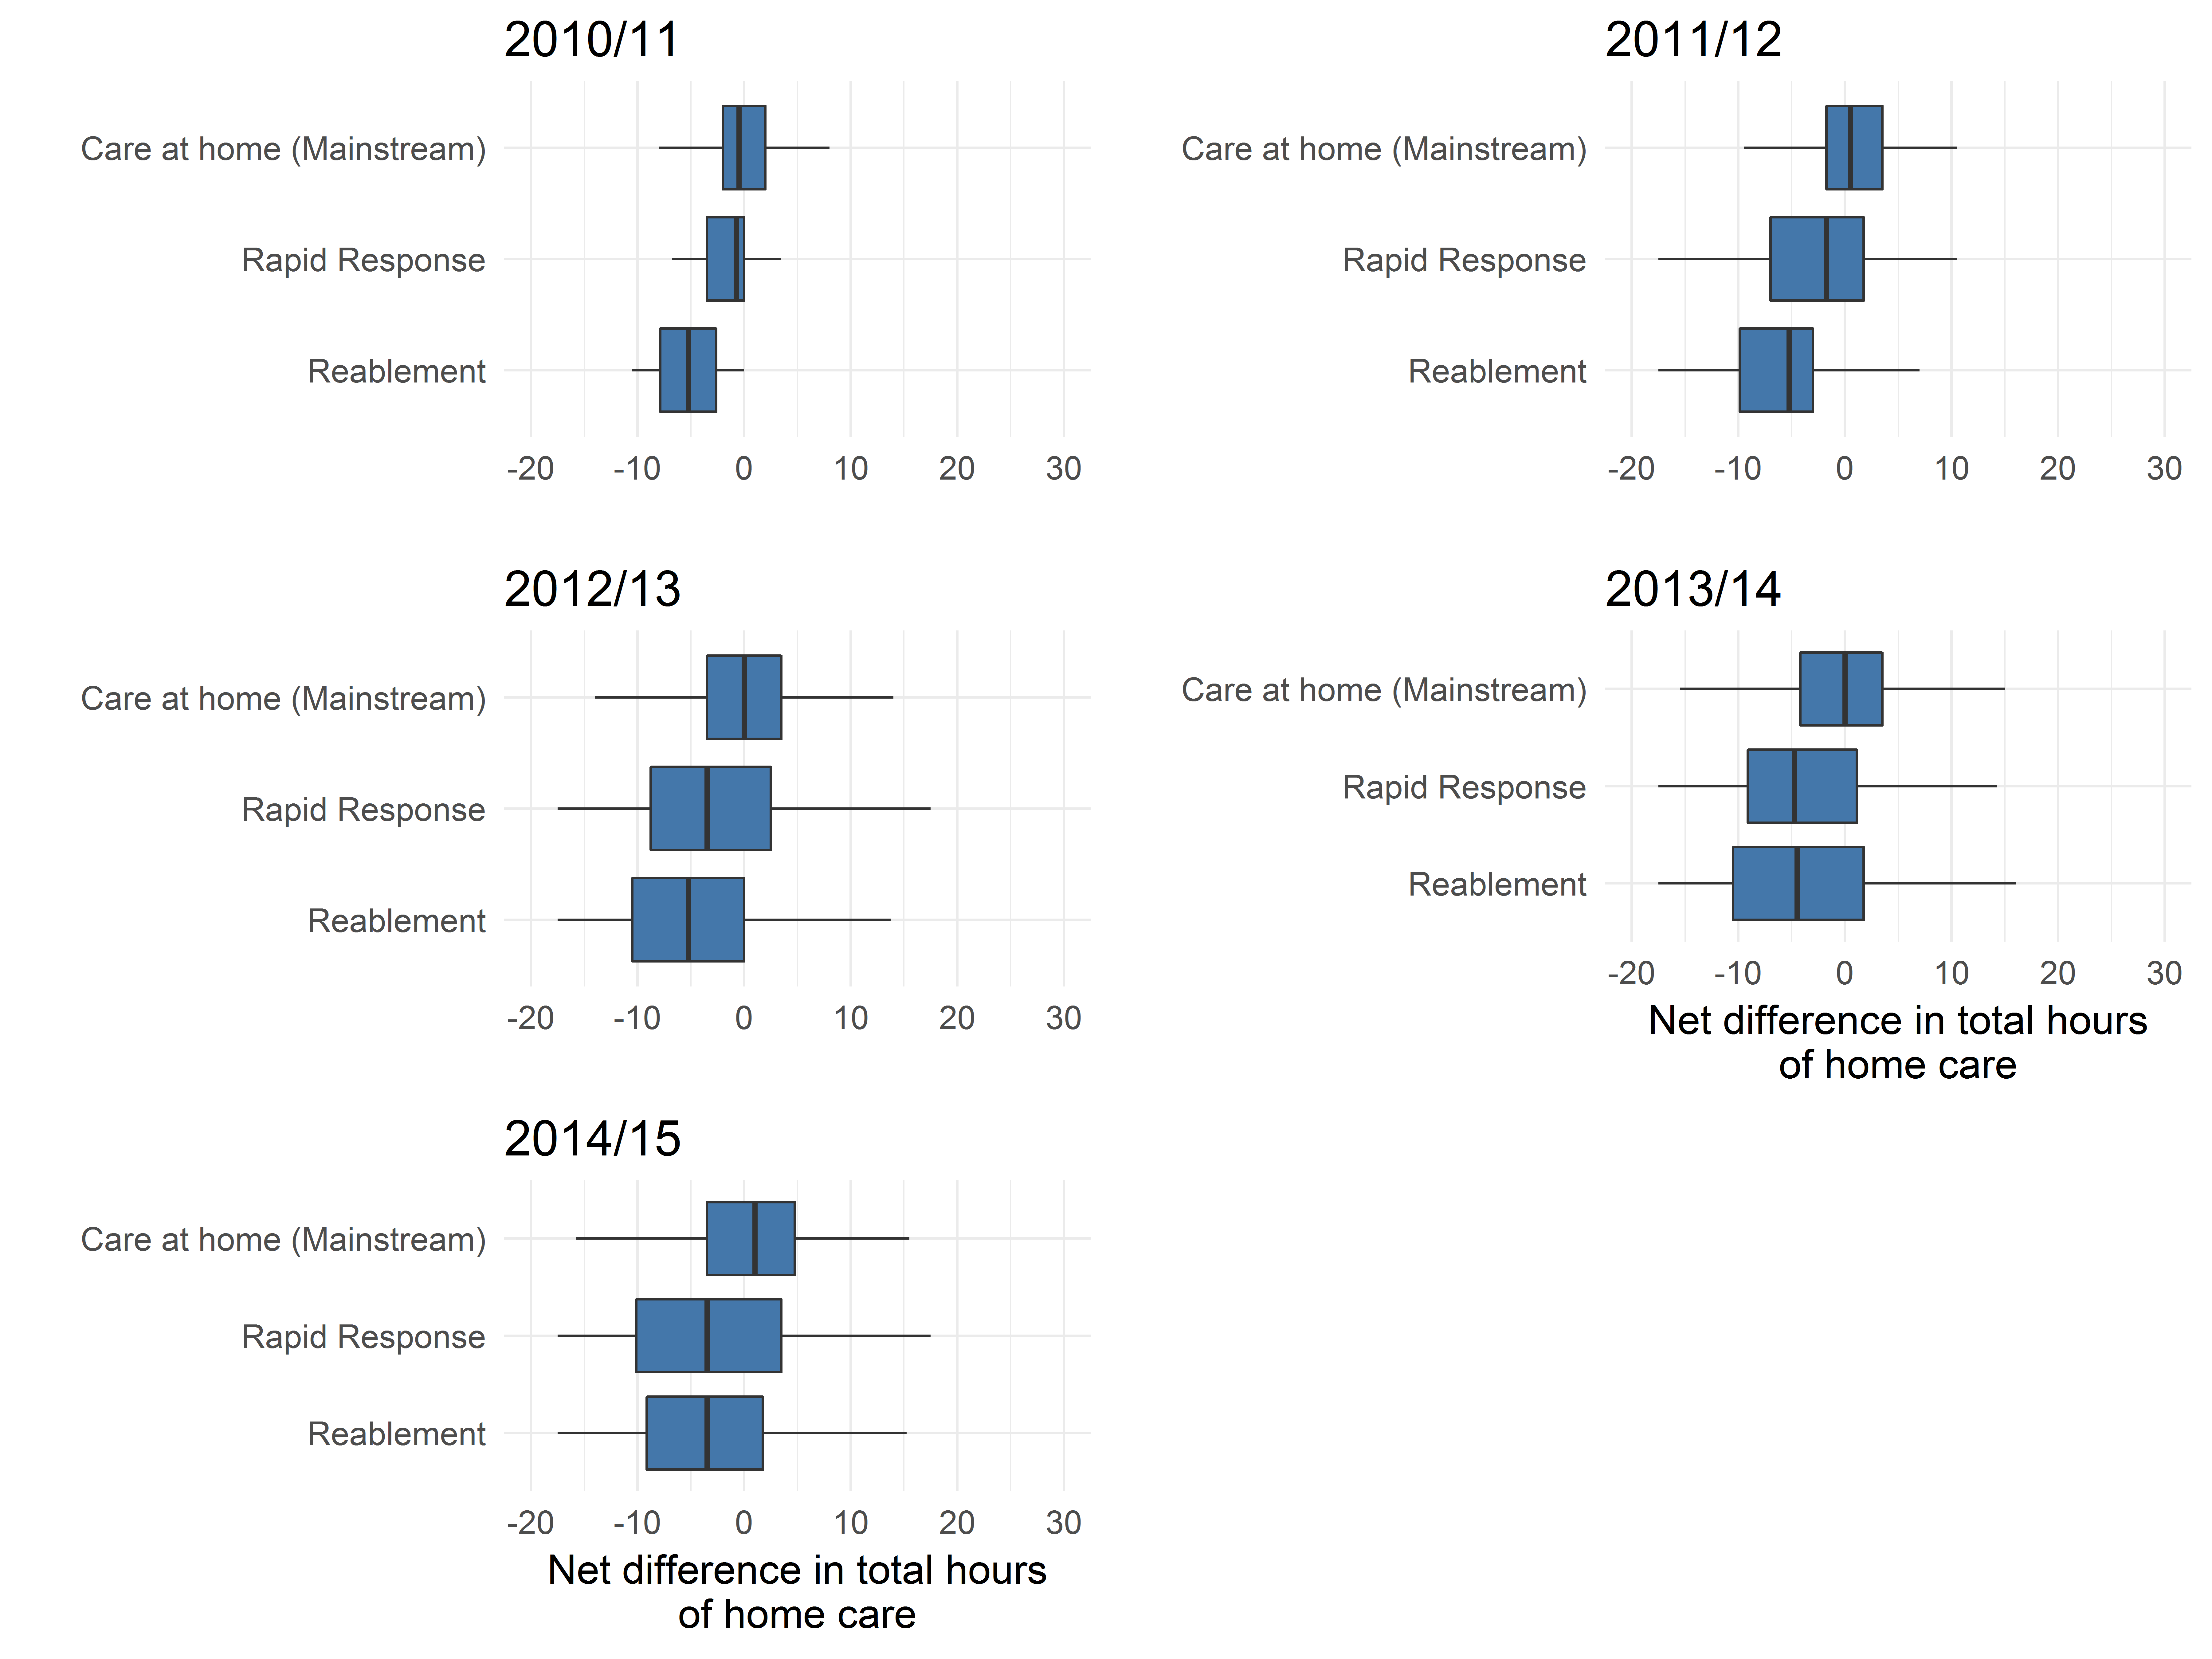
\includegraphics[]{figures/chapter-renf/10-net-diff-plot.png}
    \label{fig:renf-net-diff}
\end{figure}

\FloatBarrier
\subsection{Multi-census}\label{subsec:renf-multi-census}

\begin{table}[h]
\centering
\caption{Proportion of individuals captured by census and hypothetical multi-census in each financial year}
\label{tab:renf-multi-census}
\resizebox{\textwidth}{!}{%
\begin{tabular}{@{}lccccc@{}}
\toprule
\textbf{Financial Year} & \textbf{\begin{tabular}[c]{@{}c@{}}Total receiving\\ home care (n)\end{tabular}} & \textbf{\begin{tabular}[c]{@{}c@{}}Captured by\\ census (\%)\end{tabular}} & \textbf{\begin{tabular}[c]{@{}c@{}}Captured by six-monthly\\ census (increase) (\%)\end{tabular}} & \textbf{\begin{tabular}[c]{@{}c@{}}Captured by four-monthly\\ census  (increase) (\%)\end{tabular}} & \textbf{\begin{tabular}[c]{@{}c@{}}Captured by three-monthly\\ census (increase)(\%)\end{tabular}} \\ \midrule
2006/07 & 2435 & 62.1 & 75.5 (13.4) & 80.9 (18.8) & 84.2 (22.1) \\
2007/08 & 2465 & 60.7 & 74.5 (13.8) & 80.1 (19.4) & 83.2 (22.4) \\
2008/09 & 2438 & 61.7 & 75.0 (13.3) & 81.3 (19.6) & 84.5 (22.8) \\
2009/10 & 2428 & 61.9 & 75.5 (13.7) & 81.1 (19.2) & 83.9 (22.0) \\
2010/11 & 2157 & 57.8 & 72.8 (15.0) & 82.9 (25.1) & 85.8 (28.0) \\
2011/12 & 2096 & 59.1 & 73.4 (14.3) & 78.9 (19.8) & 82.6 (23.5) \\
2012/13 & 2381 & 57.0 & 68.2 (11.3) & 73.9 (16.9) & 77.8 (20.8) \\
2013/14 & 2599 & 54.6 & 68.1 (13.5) & 73.7 (19.1) & 78.8 (24.2) \\
2014/15 & 2763 & 56.2 & 69.7 (13.5) & 86.6 (30.4) & 87.8 (31.6) \\ \midrule
\textbf{Mean}  & 2418 & 59.0 & 72.5 (13.5) & 79.9 (20.9) & 83.2 (24.2) \\ \bottomrule
\end{tabular}%
}
\end{table}

Table \ref{tab:renf-multi-census} shows the percentage of the total
number of individuals receiving home care in each financial year that
would be captured if six-monthly, four monthly, or three-monthly census
had been conducted and the increases these would signify. A bi-annual
census would have captured an average of 72.5\% of individuals that
received home care during the study period - an average increase of
13.5\% from the census. Tri-annual census collection would have captured
an average 79.9\% of individuals (average increase of 20.9\%) whilst a
quarterly census collection would have captured an average 83.2\% of
individuals (average increase of 24.2\%).

Unsurprisingly, the largest increases are seen in the years where the
number of individuals captured by a single census are relatively low
compared to other years, in particular 2010/11, 2013/14, and 2015/16.

\section{Discussion}\label{sec:renf-discuss}

\begin{itemize}
\tightlist
\item
  60\% sample
\item
  Same type of people
\item
  Same type of packages
\item
  Different types of packages not accurately captured by categorisation?
\end{itemize}

This exploratory project has investigated the variation in packages of
care from one Scottish local authority area. It has found that figures
returned by Renfrewshire council to the SCS represent between 58.4\% and
63.7\% of the total number of individuals that the council provided home
care for in the financial years 2006/07 to 2015/16.

Counts of individuals produced by this analysis appear to be similar to
those returned by Renfrewshire Council to the SCS for the years 2006/07
to 2010/11. Thereafter, counts are slightly less. This could be due to
changes in the way data was returned to SCS from the year 2011 onwards.
There have also been changes in the criteria of which individuals should
be included in counts of home care since 2011 that could not be
replicated in this analysis.

\emph{Packages not captured by the census tend to be of much shorter
duration and have a higher intensity (measured by total hours per week)
than those packages that are seen in the census weeks.} (Maybe drop this
- need to focus more on difference in individuals rather than packages)
More recent years have seen a greater proportion of packages being
delivered for Reablement type services at the expense of Care at home
(Mainstream) type packages of care. However, reablement services only
account for a maximum of 8\% of packages captured by the census and
21.5\% not captured by the census with much lower proportions in earlier
years.

Coupled with the finding that roughly half of indivudals with ``live''
care packages during the census week have only a single package of care
in the six months pre and post census, usually with a long duration, a
picture emerges of two types of ``Care at Home (Mainstream)'' packages.
The first type are long-term packages, sometimes lasting multiple years.
The second type have much shorter duration and mirror many of the
characteristics of ``Reablement'' type packages (\emph{but I haven't
accounted for multiple packages received by one indivudal}). Whether
these packages are misclassified, or if the recent addition of
``Reablement'' packages as a care type has not yet filtered through to
data categorisation is unknown.

Returns to the SCS by local authorities do not distinguish between types
of home care but provide a value of total weekly hours of home care
only. This analysis shows that variables detailing the weekly hours of
homecare received by an indiviudal may disguise differing underlying
types of care being delivered.

\emph{Needs para on implications for research - taking into account
re-analysis of multi-packages - if duration of care is more similar then
can happily say that SCS is a good 60\% representative sample of
individuals receiving home care and can be dealt with in the same way as
any other type of cross-sectional data (with better power than most
surveys). If not, then need to quantify the error and suggest that
analysis with SCS must take account of this error. Also need to bear in
mind that \textasciitilde{}50\% of those captured by SCS will have
variation in the amount of care they receive in the year surrouning the
census but there is no way of identfying these individuls with current
SCS variables}

This analysis is limited by the fact that data was obtained from only
one local authority area. It is impossible to know if the number of
individuals captured or not by the SCS in the Renfrewshire area is
indicative of numbers across the country. Given each of the 32 local
authorities in Scotland have bespoke methods of delivering and recording
social care the findings from this analysis can not be generalised to a
national level.

Furthermore, the method of summarising data into packages of care is
subjective and may differ from the method used by Renfrewshire council.
There is some comfort in the similarity of results for some years shown
in figure \ref{fig:renf-hrs}, however there are notable differences,
particularly in later years, suggesting structural differences in
methods. The year 2010 was the first in which individual level data was
collected by the Scottish Government which may have led to different
methods of collating data. Furthermore, changes have been made at
varying intervals for what constitutes home care with differing types of
care, e.g.~Housing Support being included as home care and then
collected as a seperate type of service in later years.

Future work using this data should consider the difference in
individuals receiving care at different time intervals (e.g.~first six
months of the year). If the census week were to capture a higher
proportion of individuals in a more narrow time-frame then alternative
types of statistical analyses, such as time-to-event anlaysis, may be
possible using SCS data.\\
\textbf{longitudinal analysis}

\section{Conclusion}\label{sec:renf-conc}

Analysis of individual level social care data from Renfrewshire council
area suggests that the number of people recorded as receiving home care
by the Social Care Survey captures between 52\% and 64\% of the total
number of people that will receive home care during a financial year.
This has implications for the types of analysis that can be conducted
with SCS in data linkage projects. Those individuals receiving care in
the census week have packages of care that are broadly similar in
duration and intensity. Some reablement packages of care may be
misclassified.

\hypertarget{refs}{}
\hypertarget{ref-RN526}{}
Bache, S.M., and H Wickham. 2014. ``Magrittr:A Forward Pipe Operator for
R. R Package Version 1.5.'' Report.
\url{https://CRAN.R-project.org/package=magrittr}.

\hypertarget{ref-RN522}{}
Grolemund, G., and H Wickham. 2017. ``Lubridate:Dates and Times Made
Easy with Lubridate. R Package Version 1.6.0.'' Report.
\url{https://CRAN.R-project.org/package=lubridate}.

\hypertarget{ref-RN523}{}
Henry, L., and H Wickham. 2017. ``Purrr:Functional Programming Tools. R
Package Version 0.2.4.'' Report.
\url{https://CRAN.R-project.org/package=purrr}.

\hypertarget{ref-RN500}{}
ISD. 2017. ``Revised Source Social Care Dataset. Definitions and
Recording Guidance. (Draft Nov 2017 Version 1.4).'' Report.
\url{http://www.isdscotland.org/Health-Topics/Health-and-Social-Community-Care/docs/Proposed-SC-Definitions-Recording-Guidance-v1-3-Draft.doc}.

\hypertarget{ref-RN492}{}
NRS. 2015. ``Renfrewshire Coucnil Area - Demographic Factsheet.''
Report.
\url{https://www.nrscotland.gov.uk/files/statistics/council-area-data-sheets/renfrewshire-factsheet.pdf}.

\hypertarget{ref-RN493}{}
---------. 2016. ``Estimates of Households and Dwellings in Scotland,
2015.'' Report.
\url{https://www.nrscotland.gov.uk/files//statistics/household-estimates/house-est-15/15house-est-cor.pdf}.

\hypertarget{ref-RN295}{}
R-Core-Team. 2017. ``R: A Language and Environment for Statistical
Computing. R Foundation for Statistical Computing.'' Report.
\url{http://www.R-project.org}.

\hypertarget{ref-RN495}{}
Renfrewshire-Council. 2015. ``Corporate Records Management Policy.''
Report.
\url{http://www.renfrewshire.gov.uk/media/2763/Records-Management-Policy/pdf/App4-RecordsManagementPolicyv3.0-20151111.pdf}.

\hypertarget{ref-RN520}{}
Robinson, D. 2017. ``Broom: Convert Statistical Analysis Objects into
Tidy Data Frames. R Package Version 0.4.2.'' Report.
\url{https://CRAN.R-project.org/package=broom}.

\hypertarget{ref-RN498}{}
RStudio-team. 2016. ``Integrated Development for R. Rstudio, Inc.,
Boston, Ma. Version 1.0.143.'' Report.
\href{\%20http://www.rstudio.com/}{http://www.rstudio.com/}.

\hypertarget{ref-RN494}{}
Scottish-Government. 2017a. ``SIMD2016 Local Share Tool.'' Report.
\url{http://www.gov.scot/Resource/0051/00515034.xlsx}.

\hypertarget{ref-RN499}{}
---------. 2017b. ``Social Care Services, Scotland, 2017.'' Report.
\url{http://www.gov.scot/Publications/2017/12/3849/downloads}.

\hypertarget{ref-RN487}{}
---------. 2017c. ``Social Care Survey.'' Report.
\url{http://www.gov.scot/Topics/Statistics/Browse/Health/Data/HomeCare}.

\hypertarget{ref-RN521}{}
Wickham, H. 2017. ``Forcats:Tools for Working with Categorical Variables
(Factors). R Package Version 0.2.0.'' Report.
\url{https://CRAN.R-project.ork/package=forcats}.

\hypertarget{ref-RN525}{}
Wickham, H, and W. Chang. 2016. ``Ggplot2:Create Elegant Data
Visualisations Using the Grammer of Graphics. R Package Version 2.2.1.''
Report. \url{https://CRAN.R-project.org/package=ggplot2}.

\hypertarget{ref-RN524}{}
Wickham, H, and L. Henry. 2017. ``Tidyr:Easily Tidy Data with `Spread()`
and `Gather()` Functions. R Package Version 0.7.2.'' Report.
\url{https://CRAN.R-project.org/package=tidyr}.

\hypertarget{ref-RN283}{}
Wickham, Hadley, and Romain Francois. 2017. ``Dplyr: A Grammar of Data
Manipulation. R Package Version 0.7.4.'' Report.
\url{https://CRAN.R-project.org/package=dplyr}.


\end{document}
